% =============================================================================================================
% === PREAMBLE ================================================================================================
% =============================================================================================================

\documentclass[10pt]{book}
\usepackage{arabtex}
\usepackage{utf8}
\usepackage[utf8]{inputenc}
\usepackage[OT2, T1]{fontenc}
\usepackage{arabtex}
\usepackage[russian, english, magyar]{babel}
\usepackage{bookman}
\usepackage{thesis-kindle-style}
\usepackage[scaled]{helvet}
\renewcommand{\familydefault}{\sfdefault}
\usepackage{graphicx,wrapfig}
\usepackage{cite}
\usepackage{url}
\usepackage{amssymb,amsmath}
\usepackage{lipsum}% just to generate text for the example
\usepackage{indentfirst}
\usepackage{subcaption}
\usepackage{mwe}
\usepackage[pdftex,
	pdfauthor={Virágh, Tibor},
	pdftitle={Sakk-bot Verseny},
	pdfsubject={Sakk-bot Verseny},
	pdfkeywords={sakk, bot, verseny, szakdolgozat, programozás, mi, mesterséges intelligencia, alfa-béta, minimax, REST, API, chess, AI, alpha-beta, algorithm, thesis, ELTE},
	pdfproducer={Latex with hyperref, or other system},
	pdfcreator={pdflatex, or other tool}]{hyperref}

\newtheorem{definition}{Definíció}

\renewcommand{\listoffigures}{\begingroup
\tocsection
\tocfile{\listfigurename}{lof}
\endgroup}

\renewcommand{\listoftables}{\begingroup
\tocsection
\tocfile{\listtablename}{lot}
\endgroup}


% --- Code listing def -------------------------------------------------------------------

\usepackage{color}
\usepackage{listings}

\definecolor{red}{rgb}{0.6,0,0} % for strings
\definecolor{blue}{rgb}{0,0,0.6}
\definecolor{green}{rgb}{0,0.8,0}
\definecolor{cyan}{rgb}{0.0,0.6,0.6}

%\usepackage{caption}
%\DeclareCaptionFont{white}{\color{white}}
%\DeclareCaptionFormat{listing}{\colorbox{blue}{\parbox{\textwidth}{\hspace{15pt}#1#2#3}}} %changed \colorbox{8} to \colorbox{blue} cause 8 is not a color!
%\captionsetup[lstlisting]{format=listing,labelfont=white,textfont=white, singlelinecheck=false, margin=0pt, font={bf,footnotesize}}

\renewcommand{\lstlistingname}{Kódrészlet}% 
\renewcommand{\lstlistlistingname}{Kódrészletek listája}

% --- Code listing def (END) --------------------------------------------------------------

% Töltsd ki a saját szakdolgozatod adataival
\def\THESISTITLE{Sakk-bot Verseny}
\def\THESISAUTHOR{Virágh Tibor}
\def\THESISDEFENCEYEAR{2018}

\def\DEPARTMENT{Programozáselmélet és Szoftvertechnológiai Tanszék}
\def\SUPERVISOR{dr. Gregorics Tibor}
\def\SUPERVISORPOSITION{Tanszékvezető egyetemi docens}

\lstdefinestyle{sharpc}{language=[Sharp]C, frame=lr, rulecolor=\color{blue!80!black}}
\title{\THESISTITLE}
\author{\THESISAUTHOR}
\date{\THESISDEFENCEYEAR}

\begin{document}

\raggedbottom
\frontmatter
\pagestyle{empty}

\begin{titlepage}

\begin{minipage}{0.40\linewidth}

\includegraphics[scale=0.3]{img/elte-cimer}
\end{minipage}
\begin{minipage}{0.50\linewidth}
\begin{center}
Eötvös Loránd Tudományegyetem \\
Informatikai Kar \\
\DEPARTMENT
\end{center}
\end{minipage}

\hrule
\vfill

\begin{center}
\Huge
\textbf{\THESISTITLE}
\normalsize
\end{center}

\vfill

\begin{flushleft}
\textbf{\SUPERVISOR} \\
\SUPERVISORPOSITION \\

\textbf{\THESISAUTHOR} \\
Programtervező Informatikus BSc
\end{flushleft}

\vfill

\begin{center}
Budapest, \THESISDEFENCEYEAR
\end{center}

\end{titlepage}

\cleardoublepage

%place of the thesis subject registration form
\null
\vspace*{\fill}
\begin{figure}[htbp]
	\centering
	
\includegraphics[width=1.0\textwidth]{img/bots_chess.png}
	\caption{Robotok sakkoznak a Futurama \copyright című sorozat egyik epizódjában.}
	\label{fig:bots_chess}
\end{figure}
\vspace*{\fill}
\null
\cleardoublepage
% table of contents
\renewcommand{\contentsname}{Tartalomjegyzék}
%\tableofcontents

\pagestyle{plain}
\setcounter{page}{1}




% ============================================================================================================
% === ÖSSZEFOGLALÁS ==========================================================================================
% ============================================================================================================
\mainmatter
\newpage
\part{Bevezető}
\chapter{A dolgozatról}
\section{A dolgozat célja}
A dolgozat célja a mesterséges intelligencia kurzuson bemutatott \textbf{„kétszemélyes, teljes információjú, diszkrét, véges és determinisztikus, zéró-összegű, játékok”} algoritmusainak bemutatása a gyakorlatban, illetve az érdeklődőbb hallgatók bevonása egy olyan játékba, melyen keresztül elmélyíthetik tudásukat ezen algoritmusokból.

E célból a (normál) sakkot vesszük alapul, mely elég bonyolult ahhoz, hogy látványos eredményeket láthassunk, a legtöbben ismerik a szabályait, illetve egy klasszikus példája a fent nevezett játékok halmazának.

A dolgozat "mellékterméke" egy olyan \textit{API interface}, melyhez kapcsolódva nem csak mesterséges intelligenciát megvalósító programok, hanem "sima", emberi játékosok által is használható kliens is írható, így a téma iránt nem érdeklődők is kipróbálhatják magukat például egy mobilalkalmazás vagy egy asztali Windows / Linux alapú kliens megírásában, illetve tapasztalatra tehetnek szert az elosztott rendszerek működésében és az aszinkron programozás felettéb érdekes és néha nagy fejfájást okozó működésében is.

\section{A dolgozat felépítése}
A dolgozat három fő részből áll: jelen bevezető, a fejlesztői és a felhasználói dokumentáció.
A fejlesztői dokumentáció négy fő részre tagozódik: \textbf{"elemzés"}, \textbf{"tervezés"}, \textbf{"megvalósítás"} és \textbf{"tesztelés"} - míg a felhasználói dokumentáció a programcsomag alkalmazásai mentén van szétvágva, és mindegyiknél szót ejt a \textbf{telepítésről}, \textbf{használatról} illetve a \textbf{karbantartásról}.
A dolgozat végén kiegészítésként a függelék tartalmaz néhány a megértést segítő információt a dolgozattal kapcsolatban, illetve néhány érdekességet, tapasztalatokat.




% ============================================================================================================
% === FELHASZNÁLÓI DOKUMENTÁCIÓ ==============================================================================
% ============================================================================================================
\newpage
\part{Felhasználói Dokumentáció}

\chapter{Szerver}
\section{Telepítés}
A kiszolgáló telepítéséhez Windows környezetben a következő előfeltételek szükségesek:
\begin{itemize}
	\item Telepített IIS,
	\item Telepített .NET Core 2.1 runtime,
	\item Telepített .NET Core Hosting Bundle,
	\item MSSQL adatbázis,
	\item A klienseknek pedig .NET framework 4.7.2, ami be van építve a telepítőjükbe.
\end{itemize}
Ezen előfeltételek telepítéséről további információk a \href{https://docs.microsoft.com/en-us/aspnet/core/host-and-deploy/iis/?view=aspnetcore-2.2}{Microsoft oldalán} található.
\subsection{Fejlesztéshez, lokálisan}
\noindent Lokális telepítés lépései Visual Studio-ban: \\
\noindent \textbf{1.} Solution megnyitása Visual Studio-ban majd "Service" projekt startup projektként való beállítása: \\
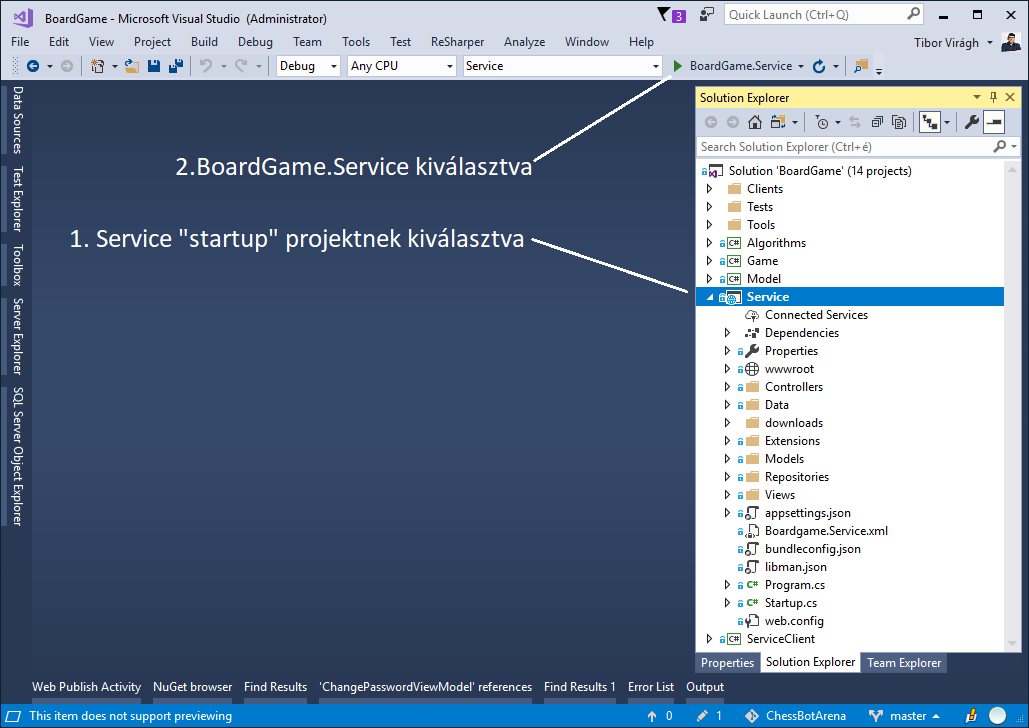
\includegraphics[width=1.0\textwidth]{img/server_dev_run_1.png} \\

\noindent \textbf{2.} Build. \\
Ekkor a Visual Studio létrehozza a site-os az IIS-ben. \\

\noindent \textbf{3.} Application pool létrehozása ("Core") a .NET core-os projekthez. A beállításokat a kép mutatja: \\
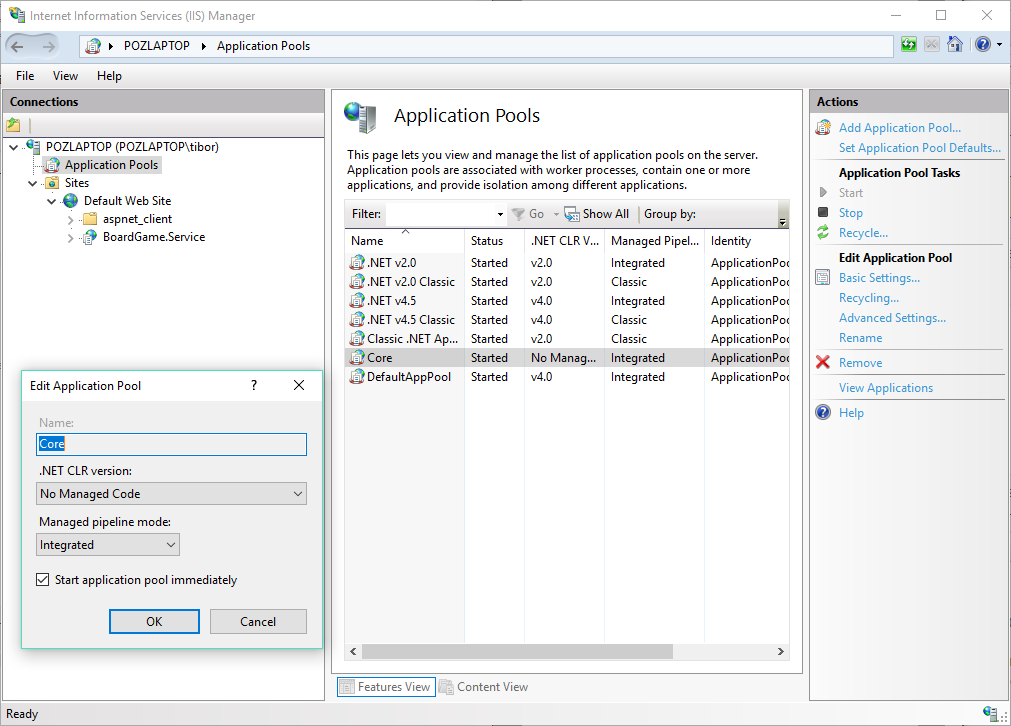
\includegraphics[width=1.0\textwidth]{img/server_dev_run_2.png} \\

\noindent \textbf{4.} Site application pool-jának beállítása az újonnan létrehozottra.
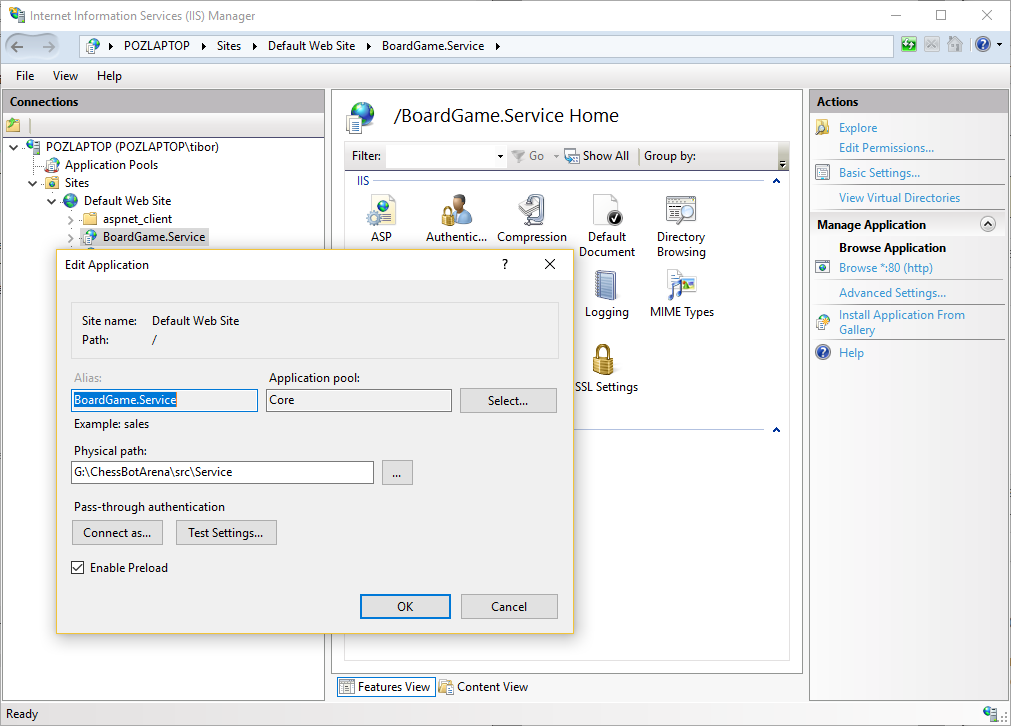
\includegraphics[width=1.0\textwidth]{img/server_dev_run_3.png} \\

\noindent \textbf{5.} Környezeti változók beállítása \\
A projektben találhatók példa konfigurációs file-ok, mint például a \texttt{appsettings.json} file. Ezekbe behelyettesíthető például az adatbázis connection string, de ez esetben fennáll a veszélye annak, hogy véletlen bekerülnek a jelszavaink egy GIT repository-ba. Ezért tanácsos helyi környezeti változókba menteni. Példa:
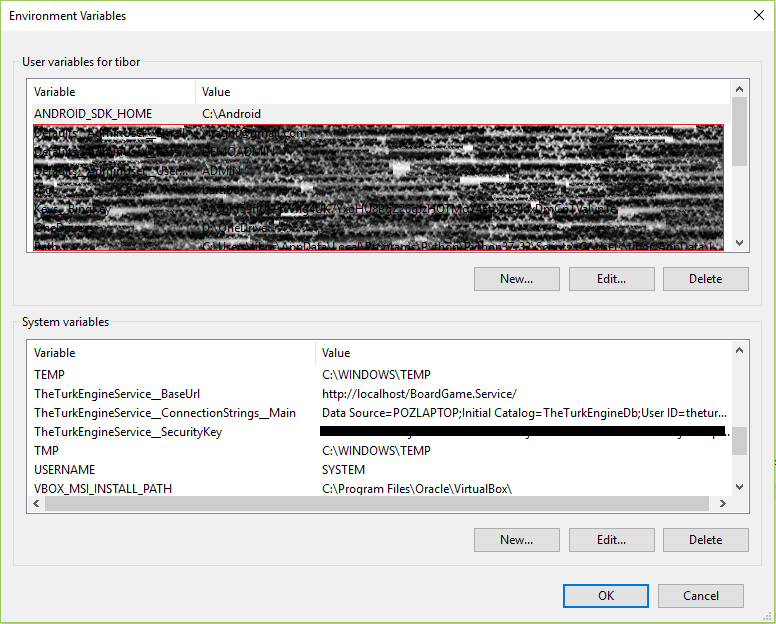
\includegraphics[width=1.0\textwidth]{img/server_dev_run_4.png}
\begin{itemize}
	\item \textbf{TheTurkEngineService\_\_BaseUrl} Ide kerül a szerver címe.
	\item \textbf{TheTurkEngineService\_\_ConnectionStrings\_\_Main} Ide kerül a connection string.
	\item \textbf{TheTurkEngineService\_\_SecurityKey} Ide kerül a privát kulcs, amivel aláírja a szervíz a JWT tokeneket.
\end{itemize}

\noindent \textbf{6.} Build és futtatás \\
Ha minden jól megy, akkor a böngészőben meg kell jelennie a frontend-nek: \\
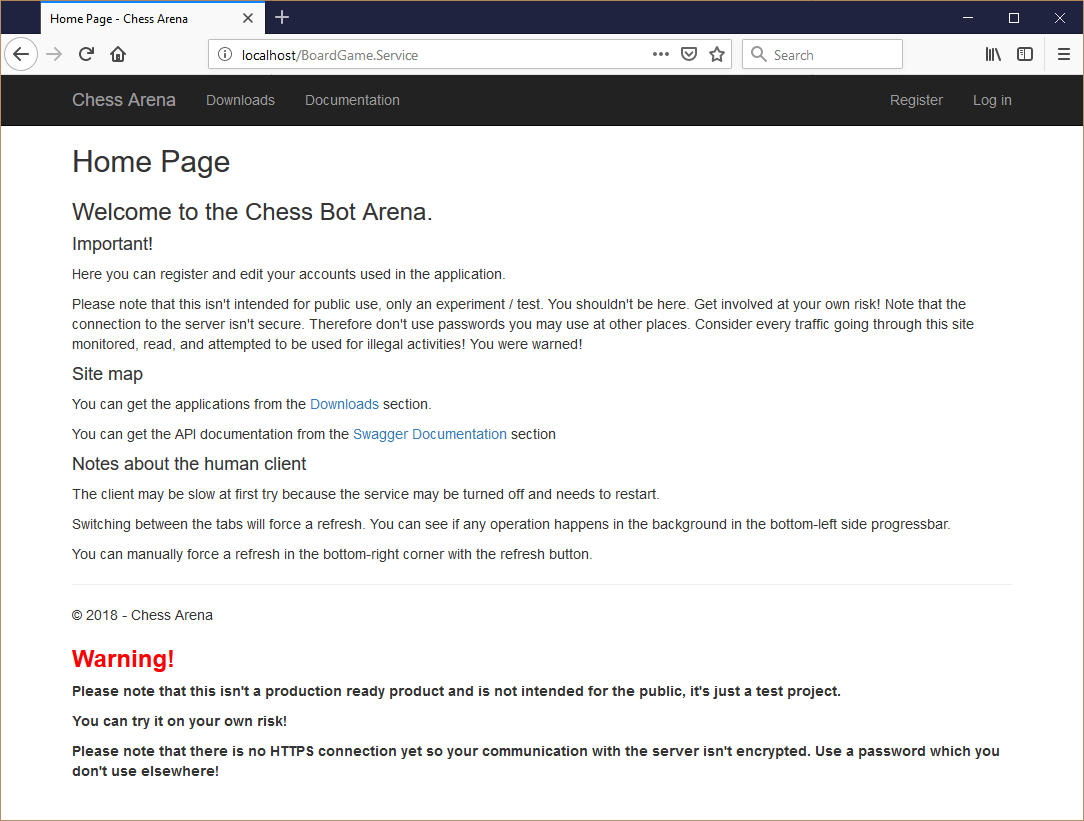
\includegraphics[width=1.0\textwidth]{img/server_dev_run_5.png} \\

\noindent \textbf{7.} Hiba esetén ellenőrizendő:
\begin{itemize}
	\item IIS-ben megfelelő application pool van-e beállítva?
	\item IISRESET futtatása adminisztátori parancssorban
	\item Windows Event Viewer tartalmazhat információt a hiba forrásáról
\end{itemize}

\subsection{Távoli szerverre}
\noindent \textbf{1.} Solution megnyitása Visual Studio-ban \\

\noindent \textbf{2.} Jobb klikk a Service projekten, majd "Publish" kiválasztása. \\

\noindent \textbf{3.} Publish ablakban szervernek megfelelő beállítások kiválasztása. Példa: \\
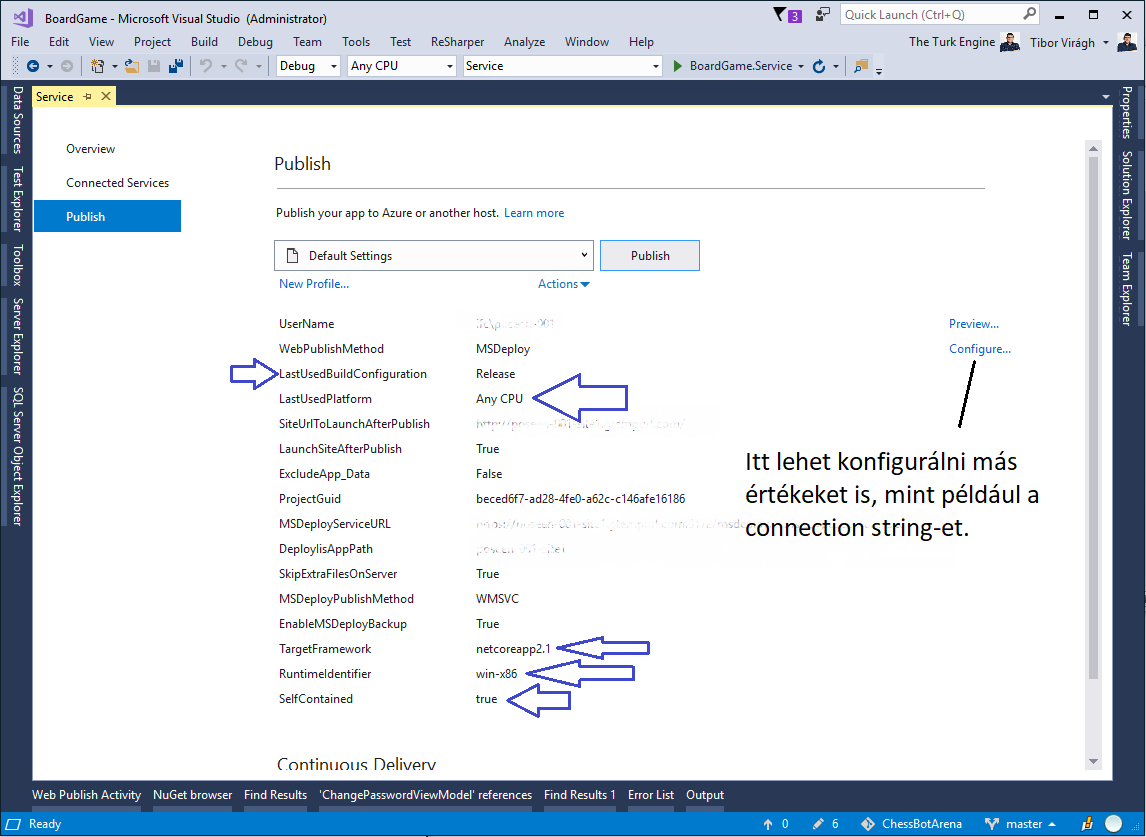
\includegraphics[width=1.0\textwidth]{img/server_prod_run_6.png} \\

\noindent \textbf{4.} Publish futtatása \\

\noindent \textbf{5.} Belépés szerverre, web.config és appsettings.json ellenőrzése. \\
Ezek módosítása ha szükséges, vagy környezeti változók használata. (Ekkor appsettings.json file törlése.)

\noindent \textbf{6.} Ha szükséges, site újraindítása. \\

\noindent \textbf{7.} Hiba esetén ellenőrizendő:
\begin{itemize}
	\item Távoli IIS-ben megfelelő application pool van-e beállítva?
	\item Távoli gépen IISRESET futtatása adminisztátori parancssorban
	\item Távoli Windows Event Viewer tartalmazhat információt a hiba forrásáról
\end{itemize}

\section{Használat}
A használati útmutató már nem csak rendszergazdáknak és a fejlesztőknek, hanem az átlagfelhasználóknak is szól.
\subsection{Regisztráció}
Az alkalmazást nem lehet regisztráció nélkül használni. Regisztráció lépései:\\

\noindent \textbf{1.} Register gombra kattintás, majd adatok megadása \\
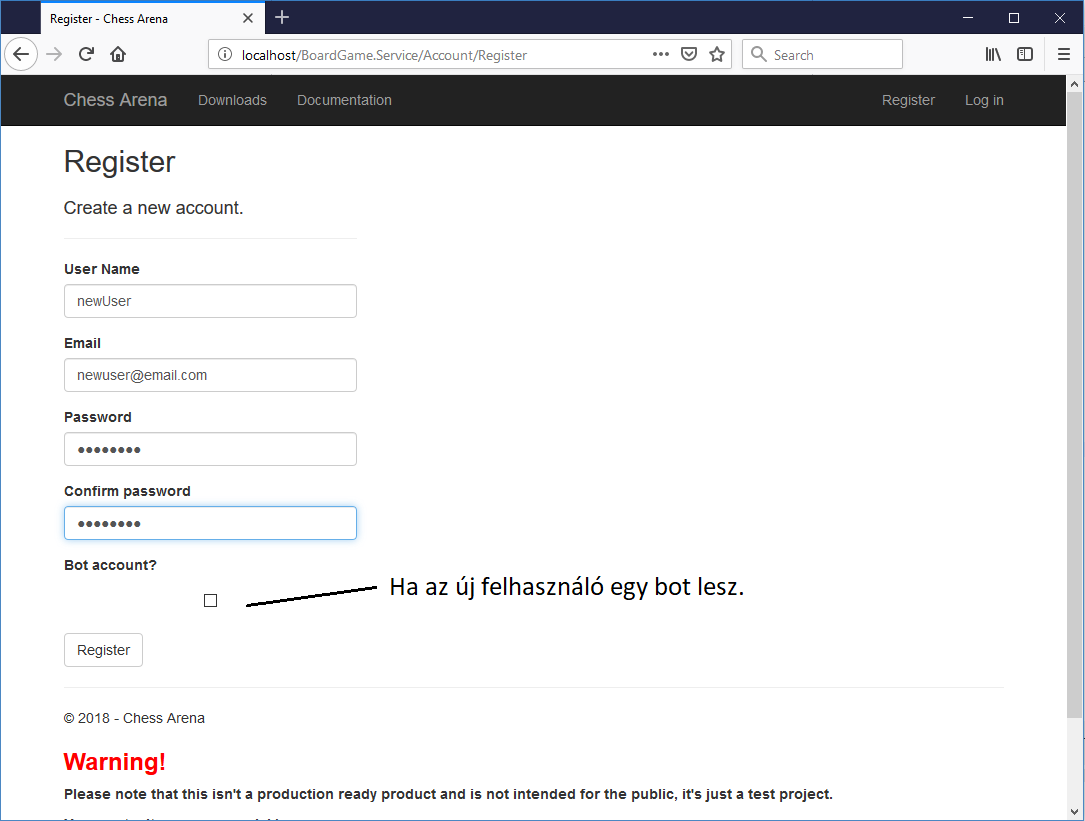
\includegraphics[width=1.0\textwidth]{img/service_register.png} \\
A jelszónak tartalmaznia kell kis és nagy betűt, egy számot és valamilyen jelet.\\
A "Bot account" alatti checkbox akkor használandó, ha egy olyan felhasználót akarunk regisztrálni, amely botként lesz nyílvántartva. \\
Ha minden rendben volt, akkor a rendszer bejelentkezteti az új felhasználót és a saját adatainak oldalára visz: \\
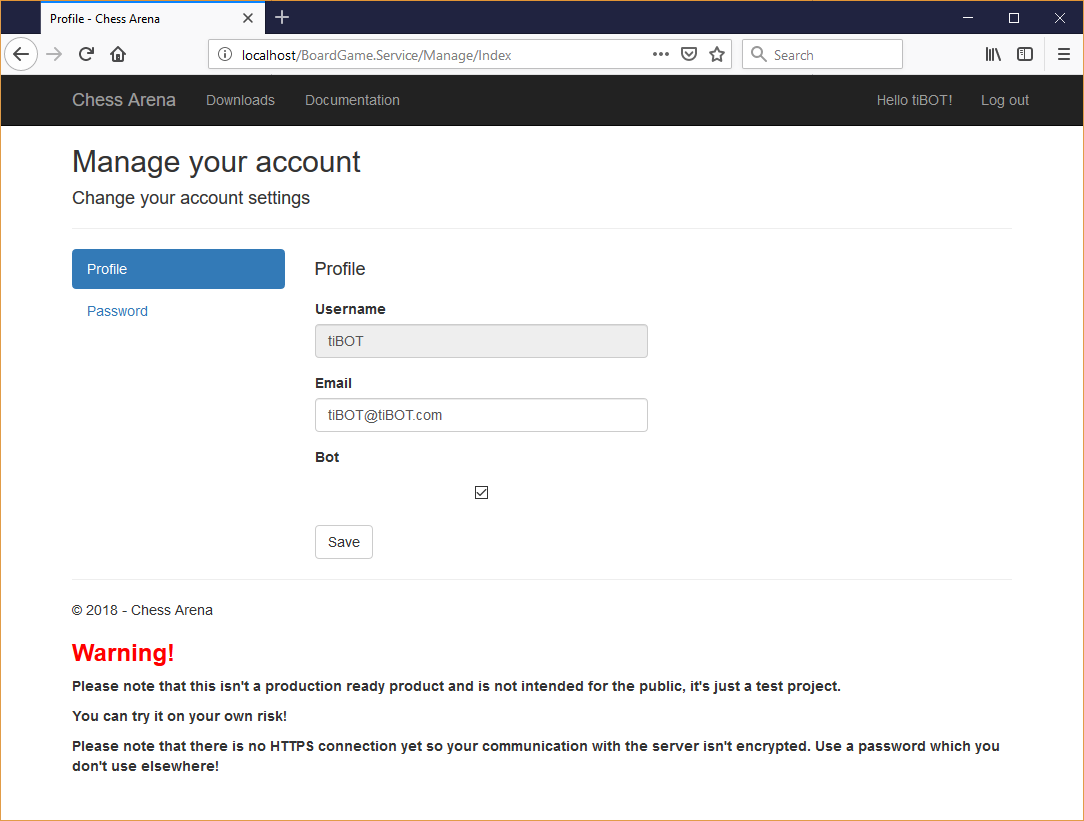
\includegraphics[width=1.0\textwidth]{img/service_account.png} \\
Ezen a képernyőn lehet módosítani a jelszót, e-mail címet, illetve azt, hogy a felhasználó robot-e.

\chapter{Játékkliens}
\section{Telepítés}
\noindent \textbf{1.} A weboldalon kattintás "Downloads" gombra, majd a megfelelő verzió letöltése \\
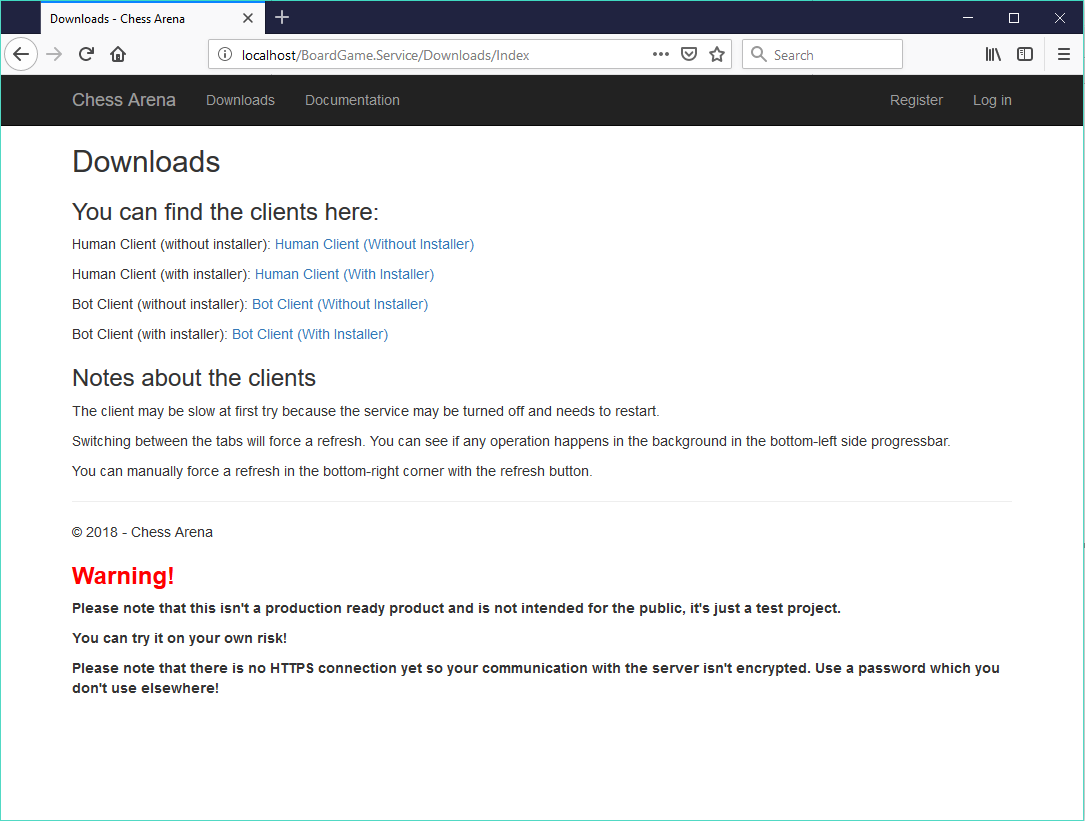
\includegraphics[width=1.0\textwidth]{img/service_downloads.png} \\
\noindent \textbf{2.} A "Without Installer" verzióban csak a futáshoz szükséges file-ok vannak betömörítve. Ezt a ZIP file-t letöltve és kitömörítve el lehet indítani a klienst. \\
A "With Installer" verzió tartalmazza a telepítőt, amely installálja a .NET Framework 4.7.2-es verzióját, ha az nincs még telepítve. Ehhez csak ki kell tömöríteni a file-t és a Setup.exe-t elindítani és követni az utasításokat.
\section{Használat}
\noindent \textbf{1.} Játékot elindítva a fő ablakba érkezünk, ahol be tudunk jelentkezni, majd a sikeres bejelentkezés után láthatjuk a játékosok listáját: \\
\includegraphics[width=1.0\textwidth]{img/chessClient_1.png} \\
\newpage
\noindent \textbf{2.} A második tabra átkattintva láthatjuk a meccseink listáját. Ezekre rákattintva a jobb oldalon egy kis előnézeti ablakban láthatjuk az ottani állást, illetve ezzel aktiválunk egy meccset arra, hogy a következő tabon megnézzük vagy esetleg lépjünk: \\
\includegraphics[width=1.0\textwidth]{img/chessClient_2.png} \\
\newpage
\noindent \textbf{3.} A harmadik oldal maga a játéktér. Először kiválasztjuk azt a bábut, amivel lépni szeretnénk, majd a megfelelő mezőre kattintva adjuk meg a lépést. A képernyő jobb oldalán látható lista tartalmazza az elmúlt lépéseket, illetve felette a speciális parancsokat.: \\
\includegraphics[width=1.0\textwidth]{img/chessClient_3.png} \\
\newpage
\noindent \textbf{4.}A negyedik oldalon látható az eddigi toplista. Csak azok látszódnak, akiknek már van befejezett játékuk. Ez a képernyő elérhető bejelentkezés nélkül is: \\
\includegraphics[width=1.0\textwidth]{img/chessClient_4.png} \\
\section{Hibaelhárítás}
\begin{itemize}
	\item Log fül tartalmazza minden kivétel szövegét, így innen esetlegesen meg lehet állapítani, mi romlott el.
	\item Windows Event Viewer is tartalmazhaz információkat
	\item Néha a szerver leáll ha sokáig nem érkezett kérés. Ekkor az első kérés eltarthat egy ideig. A kliensnek le kell kezelnie ezt a problémát. Ha mégsem sikerül, akkor később újra probálkozik a frissítéssel.
	\item Ha végképp nem érkezik válasz, akkor érdemes megnyitni a szerver weboldalát. Ha az nem megy, akkor maga a szolgáltatás is áll.
\end{itemize}
	

\chapter{Botkliens}
\section{Telepítés}
\noindent \textbf{1.} A weboldalon kattintás "Downloads" gombra, majd a megfelelő verzió letöltése \\
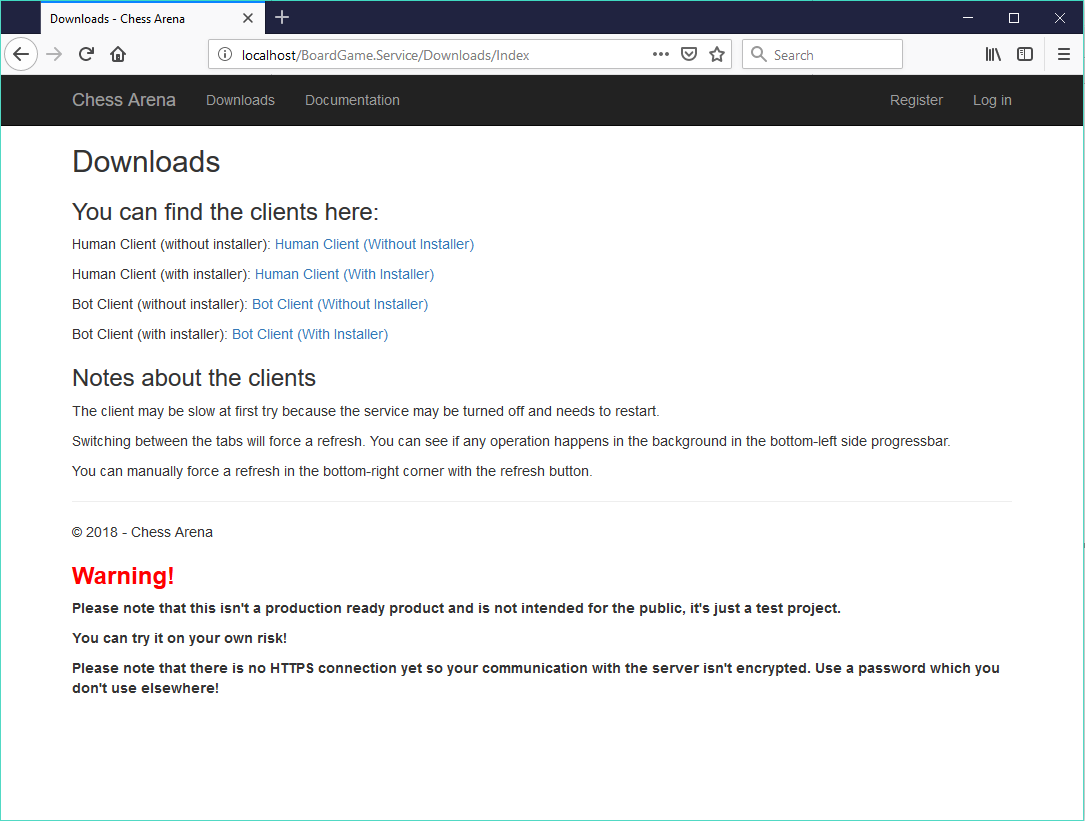
\includegraphics[width=1.0\textwidth]{img/service_downloads.png} \\
\noindent \textbf{2.} A "Without Installer" verzióban csak a futáshoz szükséges file-ok vannak betömörítve. Ezt a ZIP file-t letöltve és kitömörítve el lehet indítani a klienst. \\
A "With Installer" verzió tartalmazza a telepítőt, amely installálja a .NET Framework 4.7.2-es verzióját, ha az nincs még telepítve. Ehhez csak ki kell tömöríteni a file-t és a Setup.exe-t elindítani és követni az utasításokat.
\section{Használat}
\noindent \textbf{1.} Játékot elindítva a fő ablakba érkezünk, ahol be tudunk jelentkezni, majd a sikeres bejelentkezés után láthatjuk a játékosok listáját: \\
\includegraphics[width=1.0\textwidth]{img/botClient_1.png} \\
\newpage
\noindent \textbf{2.} A második tabra átkattintva láthatjuk a bot meccseinek listáját. Ezekre rákattintva a jobb oldalon egy kis előnézeti ablakban láthatjuk az ottani állást \\
\includegraphics[width=1.0\textwidth]{img/botClient_2.png} \\
\newpage
\noindent \textbf{3.} A harmadik oldal maga a bot vezérlőpultja. Itt állítható be, hogy milyen algoritmus, mely kiértékelő függvénnyel és milyen maximum mélységgel fusson. A tér nagy részét a bot üzeneteinek fenntartott szövegmező foglalja el. Itt látható, hogy épp mit csinál a bot. 15 másodpercenként lekéri a legfrisebb állást, majd azon meccseken, ahol ő következik és léphet, kigenerál egy lépést és elküldi. A Start/Stop gombbal indíthatjuk el / állíthatjuk le a botot. \\
\includegraphics[width=1.0\textwidth]{img/botClient_3.png} \\

\section{Hibaelhárítás}
\begin{itemize}
	\item A Log és a Bot fül tartalmaz minden információt, amelyre szükség lehet a hiba felderítésekor.
	\item Windows Event Viewer is tartalmazhaz információkat
	\item Néha a szerver leáll ha sokáig nem érkezett kérés. Ekkor az első kérés eltarthat egy ideig. A kliensnek le kell kezelnie ezt a problémát. Ha mégsem sikerül, akkor később újra probálkozik a frissítéssel.
	\item Ha végképp nem érkezik válasz, akkor érdemes megnyitni a szerver weboldalát. Ha az nem megy, akkor maga a szolgáltatás is áll.
\end{itemize}

% ============================================================================================================
% === FEJLESZTŐI DOKUMENTÁCIÓ ================================================================================
% ============================================================================================================
\newpage
\part{Fejlesztői Dokumentáció}
\chapter{Elemzés}
A megoldandó feladat egy interneten keresztül játszható sakkprogram elkészítése, melyen keresztül a játékosok egymás, illetve olyan gépi ellenfelek ("botok") ellen játszhatnak, amelyeket más játékosok készítettek. Emiatt fontos elvárás a programmal szemben, hogy emberek által könnyen használható legyen és a bot-készítő játékosok számára minden lehetséges segítség és dokumentáció a rendelkezésre álljon a feladathoz.

\section{A program felhasználási módjai}
A programcsomag felhasználási módja alapján két csoportba osztható:
\begin{itemize}
	\item \textbf{Sakk}. Ekkor a játékosok csak játszani szeretnének egymás ellen.
	
	\item \textbf{Bot-készítés.} Amikor a játékosok egy botot szeretnének kifejleszteni és azt megmérettetni más emberi és gépi ellenfelek ellen is.
\end{itemize}

Ezen két felhasználási-módnak különböző követelményei vannak.
\newpage
\section{Felhasználói esetek}
\subsection{A sakk-szolgáltatás működésével kapcsolatos elvárások}
Ebben a felhasználási helyzetben (vagy máshogy fogalmazva: a sima sakkjátékos szemszögéből) a következők a követelmények:
\subsubsection{Kliens funkcionalitása}
\begin{itemize}
	\item \textbf{Levelezési sakk.} A program működésének hasonlítania kell a levelezési sakkhoz. Nem kell teljesen valósidejűnek lennie, de bármikor le tudja tölteni az épp aktuális állást, tudjon rá reagálni és elküldeni.
	
	\item \textbf{Felhasználói fiókok.} Minden felhansználónak legyen saját fiókja.
	
	\item \textbf{Elérhető játékosok listázása.} A játékosok szeretnék látni, hogy kiket hívhatnak ki egy partira attól függetlenül, hogy az épp kiszemelt játékos be van-e jelentkezve, vagy sem.
	
	\item \textbf{Partira kihívás.} A játékosoknak lehetőséget kell adni, hogy sakkpartit tudjanak kezdeményezni egymással.
	
	\item \textbf{Partik listázása.} A játékosoknak lehetőséget kell biztosítani, hogy láthassák az eddigi játszmáikat, azok állapotát, és ki tudják választani, hogy melyikre akarnak válaszolni.
	
	\item \textbf{Sakkjátszma.} A játékosoknak az előbbiekben kijelölt sakkjátszmához lehetőséget kell biztosítani, hogy kiválaszthassák a kívánt lépést és elküldhessék. A programnak le kell ellenőriznie, hogy a lépés megfelel-e a szabályoknak.
	
	\item \textbf{Toplista.} A játékosok szeretnék látni az eddigi játszmák alapján előálló toplistát, lehetőség szerint csoportosítva: emberi játékosok, botok, vagy a kettő együtt.
\end{itemize}

% ------------------------------------------------------------------------------------------------------------
% -- Kliens - indulás 
% ------------------------------------------------------------------------------------------------------------

\begin{longtable}[c]{|c|p{7cm}|}
	\hline
	\rowcolor[HTML]{6665CD}
	\multicolumn{2}{|l|}{\cellcolor[HTML]{6665CD}{\color[HTML]{FFFFFF} \textbf{Kliens indítása}}} \\ \hline
	\endfirsthead
	%
	\multicolumn{2}{c}%
	{{\bfseries Table \thetable\ folytatása az előző oldalról...}} \\
	\hline
	\rowcolor[HTML]{6665CD} 
	\multicolumn{2}{|l|}{\cellcolor[HTML]{6665CD}{\color[HTML]{FFFFFF} \textbf{Kliens indítása}}} \\ \hline
	\endhead
	%
	\rowcolor[HTML]{CBCEFB} 
	
	%
	% --------------------------------------------------------------------------------------------------------
	%
	
	\textbf{1}
	&	Alkalmazás indítása
	\\ \nobreakhline
	
	\textbf{GIVEN} &
	A kliens telepítve van.
	\\ \nobreakhline
	
	\textbf{WHEN} &
	A felhasználó jelzi a játék indításának szándékát.
	\\
	\nobreakhline
	
	\textbf{THEN} &
	A kilens elindul és:
	\begin{itemize}
		\item Megjelenik a kliens a hitelesítési alfelülettel.
	\end{itemize} 
	\\
	\hline
	
	\caption{Kliens alapfunkciói - indítás}
	\label{userStories:client:start}\\
\end{longtable} 

% ------------------------------------------------------------------------------------------------------------
% -- Kliens - lobbi
% ------------------------------------------------------------------------------------------------------------

\begin{longtable}[c]{|c|p{7cm}|}
	\hline
	\rowcolor[HTML]{6665CD}
	\multicolumn{2}{|l|}{\cellcolor[HTML]{6665CD}{\color[HTML]{FFFFFF} \textbf{Kliens - Hitelesítési (al)felület}}} \\ \hline
	\endfirsthead
	%
	\multicolumn{2}{c}%
	{{\bfseries \thetable\ folytatása az előző oldalról...}} \\
	\hline
	\rowcolor[HTML]{6665CD} 
	\multicolumn{2}{|l|}{\cellcolor[HTML]{6665CD}{\color[HTML]{FFFFFF} \textbf{Kliens - Hitelesítési (al)felület}}} \\ \hline
	\endhead
	
	%
	% --------------------------------------------------------------------------------------------------------
	%
	
	\rowcolor[HTML]{CBCEFB} 
	\textbf{1}
	&	Kilépés
	\\ \nobreakhline
	
	\textbf{GIVEN} &
	Hitelesítési (al)felület aktív.
	\\ \nobreakhline
	
	\textbf{WHEN} &
	Kilépési szándék jelzése (majd annak pozitív megerősítése).
	\\
	\nobreakhline
	
	\textbf{THEN} &
	Alkalmazás bezárása.
	\\
	\hline
	
	%
	% --------------------------------------------------------------------------------------------------------
	%
	
	\rowcolor[HTML]{CBCEFB} 
	\textbf{2}
	&	Hitelesítés
	\\ \nobreakhline
	
	\textbf{GIVEN} &
	Hitelesítési (al)felület aktív.
	\\ \nobreakhline
	
	\textbf{WHEN} &
	\begin{itemize}
		\item Felhasználói név és jelszó megadása.
		\item Belépési szándék jelzése.
	\end{itemize}
	\\
	\nobreakhline
	
	\textbf{THEN} &
	Adatok elküldése hitelesítésre a szerverhez.
	\begin{itemize}
		\item Ha az adatok megfelelőek:
		\begin{itemize}
			\item Felhasználó beléptetése.
			\item Hitelesítési felület elrejtése.
			\item Lobbi megjelenítése
			\item Hitelesítési (al)felület elrejtése
			\item Kliens szinkronizálása a legfrissebb adatokkal.
		\end{itemize}
		
		\item Ha az adatok nem megfelelőek:
		\begin{itemize}
			\item Felhasználói tájékoztatása problémáról.
		\end{itemize}
	\end{itemize}
	\\
	\hline
	
	\caption{Kliens alapfunkciói - hitelesítési (al)felület}
	\label{userStories:client:authentication}\\
\end{longtable}

% ------------------------------------------------------------------------------------------------------------
% -- Kliens - lobbi
% ------------------------------------------------------------------------------------------------------------

\begin{longtable}[c]{|c|p{7cm}|}
	\hline
	\rowcolor[HTML]{6665CD}
	\multicolumn{2}{|l|}{\cellcolor[HTML]{6665CD}{\color[HTML]{FFFFFF} \textbf{Kliens - Lobbi}}} \\ \hline
	\endfirsthead
	%
	\multicolumn{2}{c}%
	{{\bfseries \thetable\ folytatása az előző oldalról...}} \\
	\hline
	\rowcolor[HTML]{6665CD} 
	\multicolumn{2}{|l|}{\cellcolor[HTML]{6665CD}{\color[HTML]{FFFFFF} \textbf{Kliens - Lobbi}}} \\ \hline
	\endhead
	
	%
	% --------------------------------------------------------------------------------------------------------
	%
	
	\rowcolor[HTML]{CBCEFB} 
	\textbf{1}
	&	Kilépés
	\\ \nobreakhline
	
	\textbf{GIVEN} &
	A felület aktív.
	\\ \nobreakhline
	
	\textbf{WHEN} &
	Kilépési szándék (majd annak megerősítése).
	\\
	\nobreakhline
	
	\textbf{THEN} &
	Alkalmazás bezárása.
	\\
	\hline
	
	%
	% --------------------------------------------------------------------------------------------------------
	%
	
	\rowcolor[HTML]{CBCEFB} 
	\textbf{2}
	&	Új játék kezdeményezése
	\\ \nobreakhline
	
	\textbf{GIVEN} &
	A lobbi-felület aktív.
	\\ \nobreakhline
	
	\textbf{WHEN} &
	Bejelentkezett játékosok közül leendő ellenfél kiválasztva, új játék kezdésének szándéka.
	\\
	\nobreakhline
	
	\textbf{THEN} &
	Új játék kezdeményezésére vonatkozó kérelem elküldése szervernek.
	\\
	\hline
	
	%
	% --------------------------------------------------------------------------------------------------------
	%
	
	\rowcolor[HTML]{CBCEFB} 
	\textbf{3}
	&	Partik listájának megtekintése
	\\ \nobreakhline
	
	\textbf{GIVEN} &
	A felület aktív.
	\\ \nobreakhline
	
	\textbf{WHEN} &
	Partik megtekintésének szándéka.
	\\
	\nobreakhline
	
	\textbf{THEN} &
	Partik felület mutatása.
	\\
	\hline
	\caption{Kliens alapfunkciói - lobbi}
	\label{userStories:client:lobby}\\
\end{longtable}

% ------------------------------------------------------------------------------------------------------------
% -- Kliens - partik listája
% ------------------------------------------------------------------------------------------------------------

\begin{longtable}[c]{|c|p{7cm}|}
	\hline
	\rowcolor[HTML]{6665CD}
	\multicolumn{2}{|l|}{\cellcolor[HTML]{6665CD}{\color[HTML]{FFFFFF} \textbf{Kliens - Partik listája}}} \\ \hline
	\endfirsthead
	%
	\multicolumn{2}{c}%
	{{\bfseries \thetable\ folytatása az előző oldalról...}} \\
	\hline
	\rowcolor[HTML]{6665CD} 
	\multicolumn{2}{|l|}{\cellcolor[HTML]{6665CD}{\color[HTML]{FFFFFF} \textbf{Kliens - Partik listája}}} \\ \hline
	\endhead
	
	
	%
	% --------------------------------------------------------------------------------------------------------
	%
	
	\rowcolor[HTML]{CBCEFB} 
	\textbf{1}
	&	Kilépés
	\\ \nobreakhline
	
	\textbf{GIVEN} &
	A felület aktív.
	\\ \nobreakhline
	
	\textbf{WHEN} &
	Kilépési szándék (majd annak megerősítése).
	\\
	\nobreakhline
	
	\textbf{THEN} &
	Alkalmazás bezárása.
	\\
	\hline
	
	%
	% --------------------------------------------------------------------------------------------------------
	%
	
	\rowcolor[HTML]{CBCEFB} 
	\textbf{3}
	&	Kiválasztott játék megjelenítése
	\\ \nobreakhline
	
	\textbf{GIVEN} &
	A felület aktív, partik listájában egy játék ki van választva.
	\\ \nobreakhline
	
	\textbf{WHEN} &
	Parti megtekintésének kezdeményezése.
	\\
	\nobreakhline
	
	\textbf{THEN} &
	Játékfelület mutatása.
	\\
	\hline
	\caption{Kliens alapfunkciói - partik listája felület}
	\label{userStories:client:parties}\\
\end{longtable}

\newpage
% ------------------------------------------------------------------------------------------------------------
% -- Kliens - játékfelület
% ------------------------------------------------------------------------------------------------------------

\begin{longtable}[c]{|c|p{7cm}|}
	\hline
	\rowcolor[HTML]{6665CD}
	\multicolumn{2}{|l|}{\cellcolor[HTML]{6665CD}{\color[HTML]{FFFFFF} \textbf{Kliens - játékfelület}}} \\ \hline
	\endfirsthead
	%
	\multicolumn{2}{c}%
	{{\bfseries \thetable\ folytatása az előző oldalról...}} \\
	\hline
	\rowcolor[HTML]{6665CD} 
	\multicolumn{2}{|l|}{\cellcolor[HTML]{6665CD}{\color[HTML]{FFFFFF} \textbf{Kliens - játékfelület}}} \\ \hline
	\endhead
	
	%
	% --------------------------------------------------------------------------------------------------------
	%
	
	\rowcolor[HTML]{CBCEFB} 
	\textbf{1}
	&	Kilépés
	\\ \nobreakhline
	
	\textbf{GIVEN} &
	A felület aktív.
	\\ \nobreakhline
	
	\textbf{WHEN} &
	Kilépési szándék (majd annak megerősítése).
	\\
	\nobreakhline
	
	\textbf{THEN} &
	Alkalmazás bezárása.
	\\
	\hline
	
	%
	% --------------------------------------------------------------------------------------------------------
	%
	
	\rowcolor[HTML]{CBCEFB} 
	\textbf{2}
	&	Lépés
	\\ \nobreakhline
	
	\textbf{GIVEN} &
	A felület aktív.
	\\ \nobreakhline
	
	\textbf{WHEN} &
	Lépési szándék vagy feladás/döntetlen felajánlása/döntetlen elfogadása-elutasítása ellenfélnek a sakk szabályai szerint.
	\\
	\nobreakhline
	
	\textbf{THEN} &
	Kérés elküldése szervernek, majd a játékállapot frissítése.
	\\
	\hline
	
	%
	% --------------------------------------------------------------------------------------------------------
	%
	
	\caption{Kliens alapfunkciói - játékfelület}
	\label{userStories:client:gameScreen}\\
\end{longtable}

% ------------------------------------------------------------------------------------------------------------
% -- Kliens - játékfelület
% ------------------------------------------------------------------------------------------------------------

\begin{longtable}[c]{|c|p{7cm}|}
	\hline
	\rowcolor[HTML]{6665CD}
	\multicolumn{2}{|l|}{\cellcolor[HTML]{6665CD}{\color[HTML]{FFFFFF} \textbf{Kliens - toplista}}} \\ \hline
	\endfirsthead
	%
	\multicolumn{2}{c}%
	{{\bfseries \thetable\ folytatása az előző oldalról...}} \\
	\hline
	\rowcolor[HTML]{6665CD} 
	\multicolumn{2}{|l|}{\cellcolor[HTML]{6665CD}{\color[HTML]{FFFFFF} \textbf{Kliens - toplista}}} \\ \hline
	\endhead
	
	%
	% --------------------------------------------------------------------------------------------------------
	%
	
	\rowcolor[HTML]{CBCEFB} 
	\textbf{1}
	&	Kilépés
	\\ \nobreakhline
	
	\textbf{GIVEN} &
	A felület aktív.
	\\ \nobreakhline
	
	\textbf{WHEN} &
	Kilépési szándék (majd annak megerősítése).
	\\
	\nobreakhline
	
	\textbf{THEN} &
	Alkalmazás bezárása.
	\\
	\hline
	
	%
	% --------------------------------------------------------------------------------------------------------
	%
	
	\rowcolor[HTML]{CBCEFB} 
	\textbf{2}
	&	Toplista megnyitása
	\\ \nobreakhline
	
	\textbf{GIVEN} &
	A felület aktív.
	\\ \nobreakhline
	
	\textbf{WHEN} &
	Bármely felület aktív, toplista megnyitásának szándéka.
	\\
	\nobreakhline
	
	\textbf{THEN} &
	Kérés elküldése szervernek, majd a toplista frissítése és megmutatása.
	\\
	\hline
	
	%
	% --------------------------------------------------------------------------------------------------------
	%
	
	\caption{Kliens alapfunkciói - toplista}
	\label{userStories:client:gameScreen}\\
\end{longtable}

\subsubsection{Szolgáltatás-oldal funkcionalitása}

% --------------------------------------------------------------------------------------------------------
% -- Szerver - felhasználói fiókok
% --------------------------------------------------------------------------------------------------------
\begin{longtable}[c]{|c|p{7cm}|}
	\hline
	\rowcolor[HTML]{6665CD}
	\multicolumn{2}{|l|}{\cellcolor[HTML]{6665CD}{\color[HTML]{FFFFFF} \textbf{Szolgáltatás funkciói}}} \\ \hline
	\endfirsthead
	%
	\multicolumn{2}{c}%
	{{\bfseries Table \thetable\ folytatása az előző oldalról...}} \\
	\hline
	\rowcolor[HTML]{6665CD} 
	\multicolumn{2}{|l|}{\cellcolor[HTML]{6665CD}{\color[HTML]{FFFFFF} \textbf{Szolgáltatás funkciói}}} \\ \hline
	\endhead
	
	% ----------------------------------------------------------------------------------------------------------
	%
	
	\rowcolor[HTML]{CBCEFB} 
	\textbf{1}
	&	Bejelentkezés
	\\ \nobreakhline
	
	\textbf{GIVEN} &
	A szolgáltatás elérhető.
	\\ \nobreakhline
	
	\textbf{WHEN} &
	Beérkezik egy bejelentkezési kérés egy felhasználói névvel és jelszóval.
	\\
	\nobreakhline
	
	\textbf{THEN} &
	A szolgáltatás a bejelentkezési felhasználói név és jelszó alapján visszajelez, ha sikertelen.
	Siker esetén küld egy titkosított azonosítót, amellyel a kliens tudja igazolni magát. Az azonosítónak egy idő után le kell járnia.
	Bármilyen probléma esetén jelzi a hibát.
	\\
	\hline
	
	% ----------------------------------------------------------------------------------------------------------
	%
	
	\rowcolor[HTML]{CBCEFB} 
	\textbf{2}
	&	Titkosított azonosító meghosszabbítása
	\\ \nobreakhline
	
	\textbf{GIVEN} &
	A szolgáltatás elérhető.
	\\ \nobreakhline
	
	\textbf{WHEN} &
	Beérkezik egy kérés egy azonosítóval azzal a szándékkal, hogy az érvényessége meg legyen hosszabbítva.
	\\
	\nobreakhline
	
	\textbf{THEN} &
	A szerver leellenőrzi az azonosítót, és ha még érvényes, akkor egy meghosszabbított token-t ad vissza.
	Bármilyen probléma esetén jelzi a hibát.
	\\
	\hline
	
	% ----------------------------------------------------------------------------------------------------------
	%
	
	\rowcolor[HTML]{CBCEFB} 
	\textbf{3}
	&	Szolgáltatás állapotának lekérdezése ("Health-check")
	\\ \nobreakhline
	
	\textbf{GIVEN} &
	-
	\\ \nobreakhline
	
	\textbf{WHEN} &
	Beérkezik egy kérés a szolgáltatáshoz, amelyben a kliens érdeklődik szolgáltatás státusza felől.
	\\
	\nobreakhline
	
	\textbf{THEN} &
	Ha a szolgáltatás elérhető, akkor visszajelez. (Egyébként nem.)
	\\
	\hline
	
	% ----------------------------------------------------------------------------------------------------------
	%
	
	\rowcolor[HTML]{CBCEFB} 
	\textbf{4}
	&	Játékosok lekérdezése
	\\ \nobreakhline
	
	\textbf{GIVEN} &
	A szolgáltatás fut, a kliens rendelkezik érvényes token-nel.
	\\ \nobreakhline
	
	\textbf{WHEN} &
	Beérkezik egy kérés a szolgáltatáshoz, amelyben a kliens lekéri a játékosok listáját.
	\\
	\nobreakhline
	
	\textbf{THEN} &
	A szolgáltatás visszaküldi a játékosok listáját (ha érvényes volt a token).
	Bármilyen probléma esetén jelzi a hibát.
	\\
	\hline
	
	% ----------------------------------------------------------------------------------------------------------
	%
	
	\rowcolor[HTML]{CBCEFB} 
	\textbf{5}
	&	Partik lekérdezése
	\\ \nobreakhline
	
	\textbf{GIVEN} &
	A szolgáltatás fut, a kliens rendelkezik érvényes token-nel.
	\\ \nobreakhline
	
	\textbf{WHEN} &
	Beérkezik egy kérés a szolgáltatáshoz, amelyben a kliens lekéri az aktuális játékos partijainak listáját.
	\\
	\nobreakhline
	
	\textbf{THEN} &
	A szolgáltatás visszaküldi a partik listáját ha érvényes a token.
	Bármilyen probléma esetén jelzi a hibát.
	\\
	\hline
	
	% ----------------------------------------------------------------------------------------------------------
	%
	
	\rowcolor[HTML]{CBCEFB} 
	\textbf{6}
	&	Lépés
	\\ \nobreakhline
	
	\textbf{GIVEN} &
	A szolgáltatás fut.
	\\ \nobreakhline
	
	\textbf{WHEN} &
	Beérkezik egy kérés a szolgáltatáshoz, amelyben a kliens közli, hogy melyik partin milyen lépést szeretne kezdeményezni.
	\\
	\nobreakhline
	
	\textbf{THEN} &
	A szolgáltatás ellenőrzi, majd végrehajtja és lementi a lépést, erről visszaigazolást küld a legfrisebb állással.
	Bármilyen probléma esetén jelzi a hibát.
	\\
	\hline
	
	% ----------------------------------------------------------------------------------------------------------
	%
	
	\rowcolor[HTML]{CBCEFB} 
	\textbf{7}
	&	Kihívás
	\\ \nobreakhline
	
	\textbf{GIVEN} &
	A szolgáltatás fut.
	\\ \nobreakhline
	
	\textbf{WHEN} &
	Beérkezik egy kérés a szolgáltatáshoz, amelyben a kliens közli, hogy melyik felhasználót szeretné kihívni.
	\\
	\nobreakhline
	
	\textbf{THEN} &
	A szolgáltatás ellenőrzi a kérést, majd ha rendben találja, kisorsolja hogy melyik játékos lesz a fehér, majd létrehozza a játékot és visszaküldi a meccs alapinformációit a kliensnek.
	Bármilyen probléma esetén jelzi a hibát.
	\\
	\hline
	
	% ----------------------------------------------------------------------------------------------------------
	%
	
	\rowcolor[HTML]{CBCEFB} 
	\textbf{8}
	&	Eredmények
	\\ \nobreakhline
	
	\textbf{GIVEN} &
	A szolgáltatás fut.
	\\ \nobreakhline
	
	\textbf{WHEN} &
	Beérkezik egy kérés a szolgáltatáshoz, amelyben a kliens le akarja tölteni a felhasználók aktuális pontjait. (LADDER végpont, POST metódus)
	\\
	\nobreakhline
	
	\textbf{THEN} &
	A szolgáltatás a befejezett játékok alapján kiszámolja és visszaküldi a felhasználók toplistáját.
	Bármilyen probléma esetén jelzi a hibát.
	\\
	\hline
	
	\caption{Szolgáltatás alapfunkciói}
	\label{userStories:server:api}\\
\end{longtable} 

\subsubsection{Bot-készítés}
A bot elkészítésének segítéséhez magas fokú \textbf{dokumentáltáság} és a lehető legtöbb segítség megadása szükséges a programozók számára könnyen felhasznáéható könyvtárak illetve példák formájában:
\begin{itemize}
	\item \textbf{Dokumentáció} a szolgáltatás és a könyvtárak használatáról.
	\item \textbf{Könyvtárak} melyek segíthetik a programozó munkáját:
	\begin{itemize}
		\item Játék-modellezését segítő könyvtár,
		\item Mesterséges Intelligencia készítését segítő könyvtár(ak).
	\end{itemize}
\end{itemize}

\section{A sakktábla információhiánya}\label{A Sakktábla információhiánya}
A sakk szabályait nem részleteznénk, ismertnek tételezzük fel, illetve az interneten könnyen hozzáférhető, mint például a \href{http://www.sakk.hu/help/sakk_szabalyok.html}{Sakk.hu} ~\cite{chessrulessakkhu} oldalon. Néhány fontos dolog azért megjegyzendő, amely kissé megbonyolítja a sakk szabályait.

\textit{Egy volt munkahelyemen dekoráció gyanánt ki volt rakva egy sakktábla bábukkal. Ezt az emberek elkezdték használni: kinyomtattak egy papírt, egyik oldalára azt, hogy "fehér jön" a másik oldalára pedig azt, hogy "fekete jön". Ha valakinek volt kedve és ideje, odamehetett, elgondolkodhatott a lépésen, majd miután lépett, megfordította a papírt és várták, hogy valaki lépjen.}

Felmerülhet a kérdés: a meccs "előtörténetének" ismerete nélkül vajon csak a tábla ismeretével kiszámítható-e az összes lehetséges lépés? Ha valaki odalép ehhez a sakktáblához, meg tudja-e mondani az összes lehetséges lépést? A rövid válasz: \textbf{nem}. A hosszú válasz: \textbf{igen, de az már egy egyszerűsített sakk}. Vannak különleges lépések, amelyekhez kell ismerni a parti addigi alakulását is (mikor lehet feladni a játékot, mikor áll be automatikusan döntetlen), illetve ha az előző lépések nem is, de valamilyen cimke a bábukon is kell vagy kellhet, például a sáncolás, vagy az \textit{en passant} lépés felismeréséhez.

Első példaként vegyük szemügyre a sáncolást. Ekkor láthatjuk, hogy a benne résztvevő bábuknak nem elég a helyükön lenni, de az is elvárás tőlük, hogy nem is mozoghattak előtte. Ezt meg lehet állapítani az előző lépések vizsgálatával, vagy ha gyorsítani akarunk ezen, akkor egy cimke ráragaszásával arra bábura, amely elmozdult a játszma során.

Második ilyen példa a kevésbé ismert "\textit{en passant}" ütés. Ez akkor következik be, amikor az ellenfél az egyik gyalogjával kettőt lép előre pont a mi gyalogunk mellé. Ebben az esetben a következő (és csakis a következő) körben leüthető úgy, mintha nem kettőt, csak egyet lépett volna eredetileg előre. Viszont fontos, hogy ha nem ütjük le, akkor a következő körben ezt már nem tehetjük meg. Ez esetben is használható a "cimkézés", amelyet a lépés után rárakunk, de ha a következő körben az ellenfél nem üti le, akkor levesszük róla.

Harmadik érdekes szabály az, hogy ha többször fordul elő ugyanaz az állapot, akkor a játékosok felajánlhatnak döntetlent a másiknak. Ehhez viszont ismerni kell az előző lépéseket, a táblára "simán csak ránézve" ezt a szabályt sem lehet alkalmazni. Ebben az esetben a cimkézés már nem elég, ehhez a szabályhoz már kell az előtörténet ismerete is.

\newpage
\chapter{Tervezés}
Az előzőekből látható, hogy két nagy részre bontható programcsomagról van szó. Az egyik a \textbf{kliens} oldal a másik a \textbf{szolgáltatást nyújtó} oldal. Erre egy sima szerver-kliens architektúra alkalmazása megfelelőnek tünik: (\ref{fig:highLevelArchitecture} ábra.)

\begin{figure}[htbp]
	\centering
	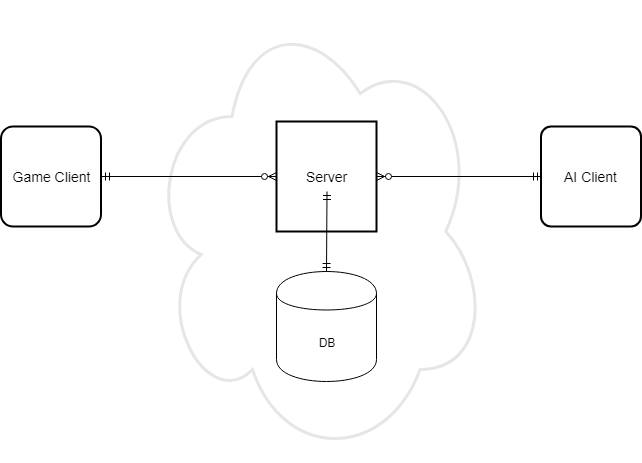
\includegraphics[width=1.0\textwidth]{img/highLevelArchitecture.png}
	\caption{Magas-szintű architektúra}
	\label{fig:highLevelArchitecture}
\end{figure}

\section{A szerver}

A szerver a következő funkciókat megvalósító végpontokkal fog rendelkezni:

\begin{itemize}
	
	\item \textbf{Felhasználó regisztrációja} \\
	Felhasználói fiókok létrehozása, kezelése. Különbséget kell tenni az emberi- és a botjátékosok között. Ez kell ahhoz, hogy később a toplista csoportosítható legyen.
	
	\item \textbf{Felhasználó nyomonkövetése.} \\
	A felhasználók belépését, kilépését, tokenek érvényességének vizsgálatát is a szerver végzi és csak akkor nyújtja a szolgáltatásokat, ha ezek rendben voltak.
	
	\item \textbf{Játékosok listája} \\
	Csak bejelentkezett felhasználók láthatják és így csak ők hívhatnak ki egy játékost.
	
	\item \textbf{Meccsek listája} \\
	Csak bejelentkezett felhasználók láthatják a saját meccseiket és csak akkor léphetnek, ha a szabályok szerint ez lehetséges.
	
	\item \textbf{Lépések ellenőrzése} \\
	Bejelentkezett felhasználó ha van kijelölt meccs, akkor a lépést a szerver ellenőrzi, hogy a sakk szabályai szerint érvényes-e. Ha igen, akkor elvégzi a parti módosítását és elmenti az új állapotot, majd a változást közvetíti a kliens felé.
	
	\item \textbf{Toplista} \\
	Bejelentkezés nélkül is elérhető, kilistázza a regisztrált játékosok eddigi eredményeit, feltéve ha vannak mások ellen befejezett meccsei.
	
	\item \textbf{Státusz} \\
	Bejelentkezés nélkül is elérhető, akkor válaszol, ha a szerver fut.
		
\end{itemize}

\subsection{A szerver felhasználói felülete}
A szervernek rendelkeznie kell felhasználói felülettel, ahol a regisztráció és felhasználói adatmódosítás elérhető, illetve innen lehet elérni különböző a játékkal kapcsolatos anyagokat is, mint például a dokumentáció, letölthető kliensek.
\subsubsection{Szerver főfelülete}
Minimalista, csak dokumentációt, letöltéseket, felhasználó regisztráció és menedzsment elérhető róla. (\ref{fig:serverUiMainScreen}. ábra)

\begin{figure}[htbp]
	\centering
	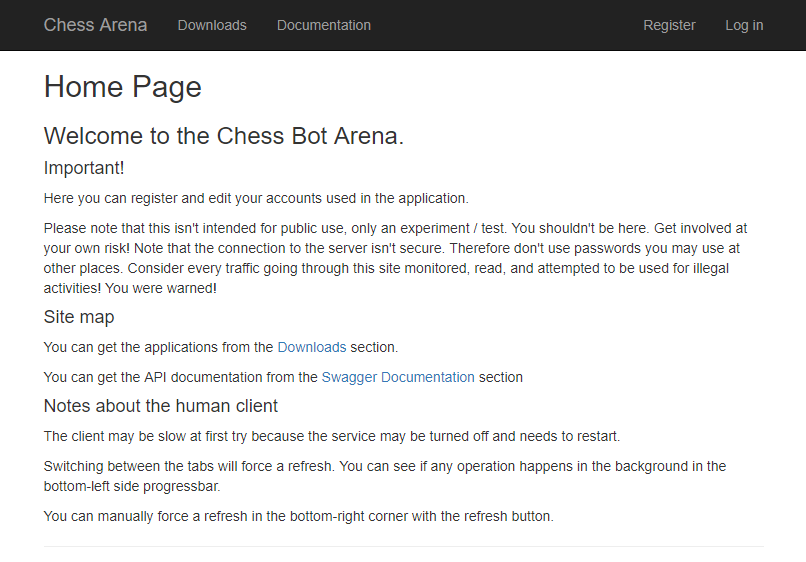
\includegraphics[width=1.0\textwidth]{img/serverUiMainScreen.png}
	\caption{Szerver fő felület}
	\label{fig:serverUiMainScreen}
\end{figure}

\subsubsection{Dokumentáció}
Az automatikusan generált, a fejlesztést segítő dokumentáció tervét mutatja a(z) \ref{fig:serverUiDocumentation}. ábra.

\begin{figure}[htbp]
	\centering
	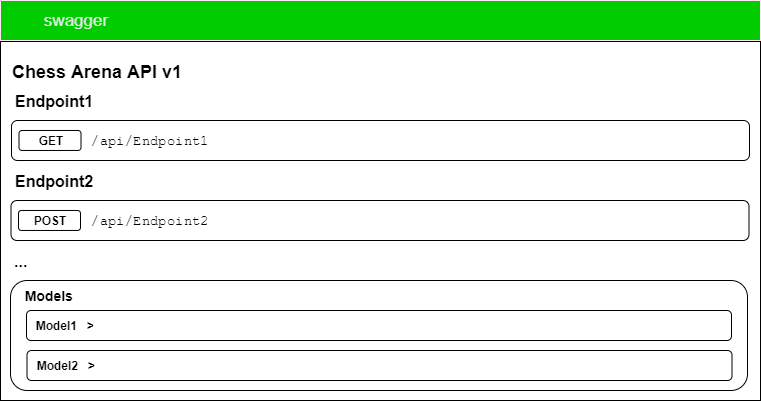
\includegraphics[width=1.0\textwidth]{img/serverUiDocumentation.png}
	\caption{Szerver - generált dokumentáció}
	\label{fig:serverUiDocumentation}
\end{figure}


\section{Játék- és botkliensek}
A klienseket ketté lehet bontani az alapján, hogy ki hozza a döntéseket. Ezek szerint lesznek \textbf{játékkliensek}, ahol emberi játékosok tudnak játszani, illetve lesznek a \textbf{botkliensek}, melyek minimális vagy semmilyen emberi beavatkozással tudnak válaszolni a bejövő kérésekre.

A két fajta kliens nem tér el túlságosan, mindkettőben kell támogatni a beléptetést, nyomonkövetést, játékinformációk szinkronizációját.

Amiben viszont eltérnek az, hogy mekkora önállóságuk van. A játékkliensnél a lépéseket az emberi felhasználó határozza meg, míg a botkliensnél egy MI algoritmus. Adódhat az ötlet, hogy a más felhasználók kihívását is automatizáljuk, de nem egyértelmű olyan megoldás implementálása, ami nem árasztja később el a játékosokat kihívásokkal, ezért ez a funkció maradhat az emberi felhasználónál.

A botkliensekből legyen lehetőség kézzel kihívni másokat, de ne tegye automatikusan. Természetesen emberi játékosok kihívhatják a botokat, azok onnantól kezdve automatikusan kell, hogy válaszoljanak a felkérésekre.
Fontos kitétel a klienseknél, hogy nem szabad leállniuk egy-egy kérésnél, mindig tudniuk kell válaszolni.

A kliensek sokfélék lehetnek, nem kívánatos egy technológiához kötni őket, ezért a szerver-kliens kapcsolatot úgy kell megtervezni, hogy bármely platformon könnyen elérhető és megvalósítható legyen.

\subsection{A kliensek működése}
A különböző tabok között szabadon válthat a felhasználó. Minden tabváltáskor történik egy frissítés, amely hatására az összes oldalon levő UI elem frissül. Természetesen a frissítés a háttérben kell, hogy történjen, a UI nem "fagyhat le".

A terveken nincs kiemelve, de mindkét kliensben van egy \textbf{Log} és egy \textbf{Read me} tab. Előbbi hibakereséskor jön majd jól, ugyanis a klienseknek nem szabad semmilyen \textit{exception}-t dobni, viszont mindent le kell logolnia. A \textit{Read me} tab tartalmazza a klienshez a hasznos tudnivalókat, figyelmeztetéseket.

A következőkben lássuk a két megvalósítandó kliens felhasználói felületének terveit. Természetesen ezek csak példák, mivel a szolgáltatás nyílt API-val kell, hogy rendelkezzen, ezért a jövőbeli fejlesztőknek bármilyen más elképzelésük is lehet, például egy BASH kliens megírása is lehetséges.

A képeken látszik, hogy a két kliens nagyon hasonlít egymáshoz hiszen funkcionalitásban is elég közel állnak egymáshoz.

\subsection{A játékkliens felhasználói felülete}
(Lásd: \ref{fig:humanClient}.ábra)

\begin{figure*}
	\centering
	\begin{subfigure}[b]{0.475\textwidth}
		\centering
		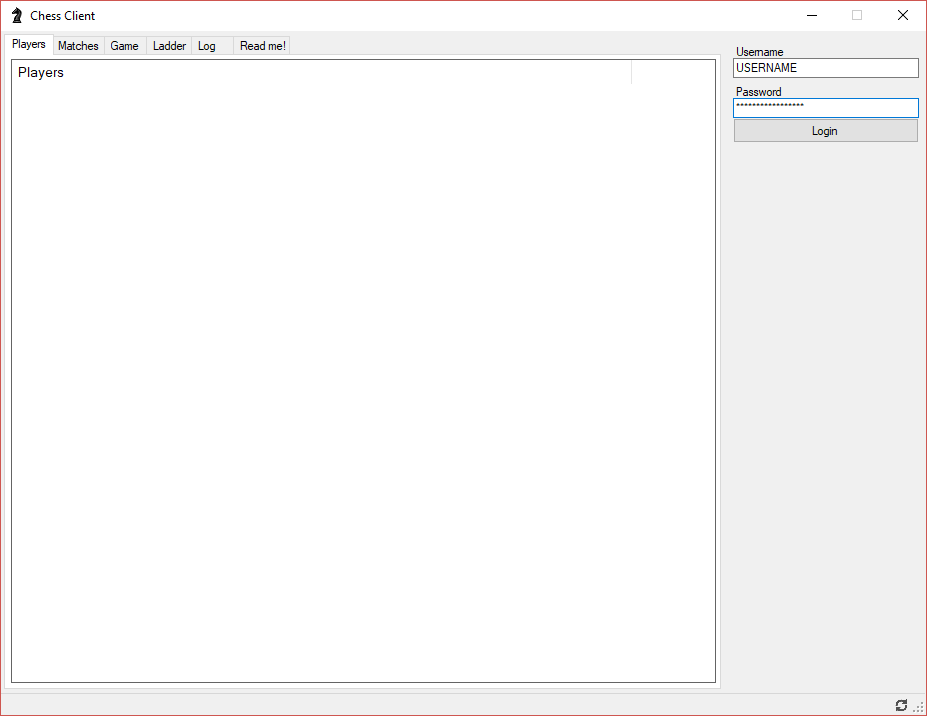
\includegraphics[width=\textwidth]{img/humanClientLogin.png}
		\caption{Belépő képernyő}
		\label{humanClientLogin}
	\end{subfigure}
	\hfill
	\begin{subfigure}[b]{0.475\textwidth}  
		\centering 
		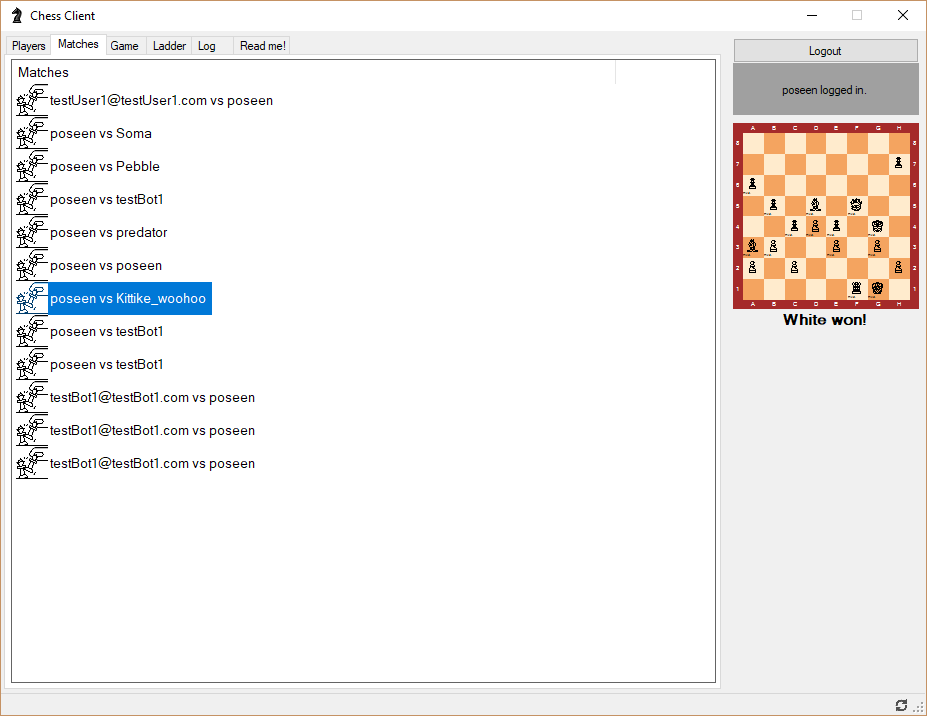
\includegraphics[width=\textwidth]{img/humanClientMatches.png}
		\caption{Partik}
		\label{fig:humanClientMatches}
	\end{subfigure}
	\vskip\baselineskip
	\begin{subfigure}[b]{0.475\textwidth}   
		\centering 
		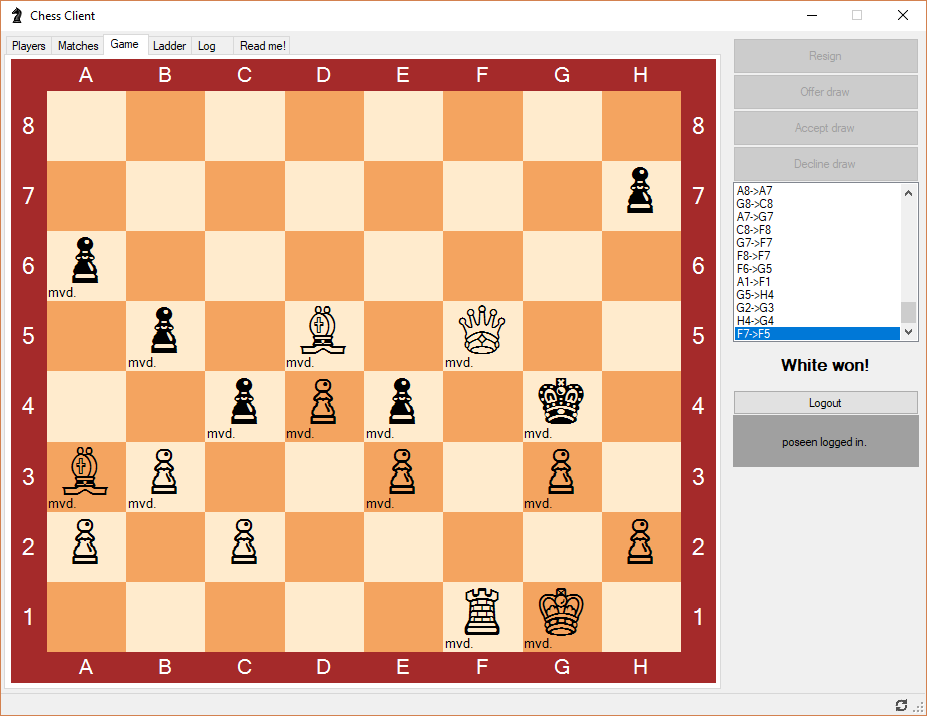
\includegraphics[width=\textwidth]{img/humanClientGame.png}
		\caption{Bot vezérlése}
		\label{fig:humanClientGame}
	\end{subfigure}
	\quad
	\begin{subfigure}[b]{0.475\textwidth}   
		\centering 
		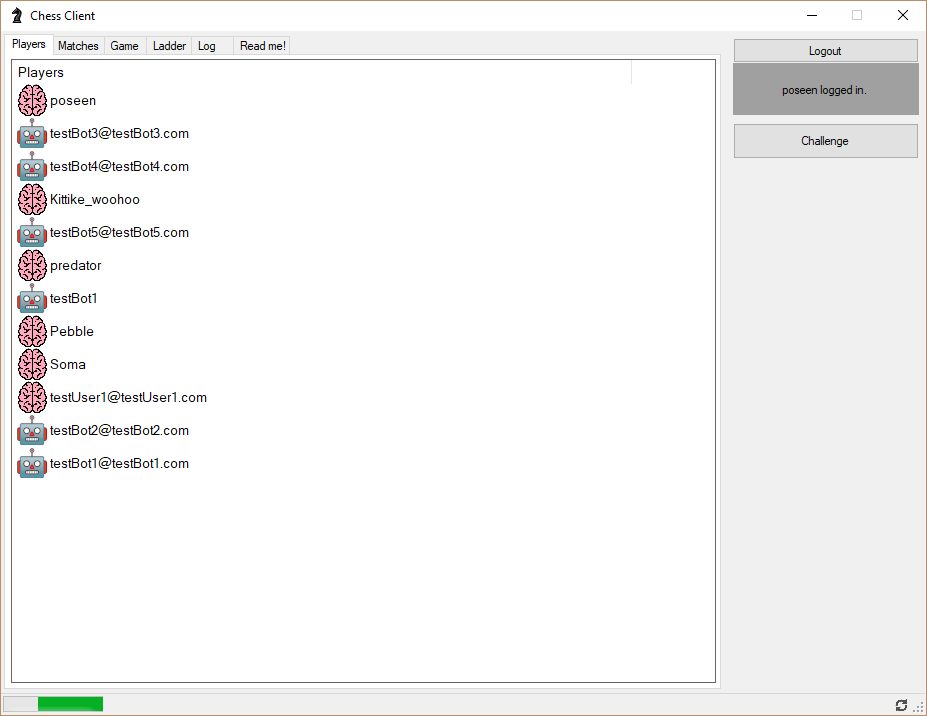
\includegraphics[width=\textwidth]{img/humanClientPlayers.png}
		\caption{Játékosok listája}
		\label{fig:humanClientPlayers}
	\end{subfigure}
	\vskip\baselineskip
	\begin{subfigure}[b]{0.475\textwidth}   
		\centering 
		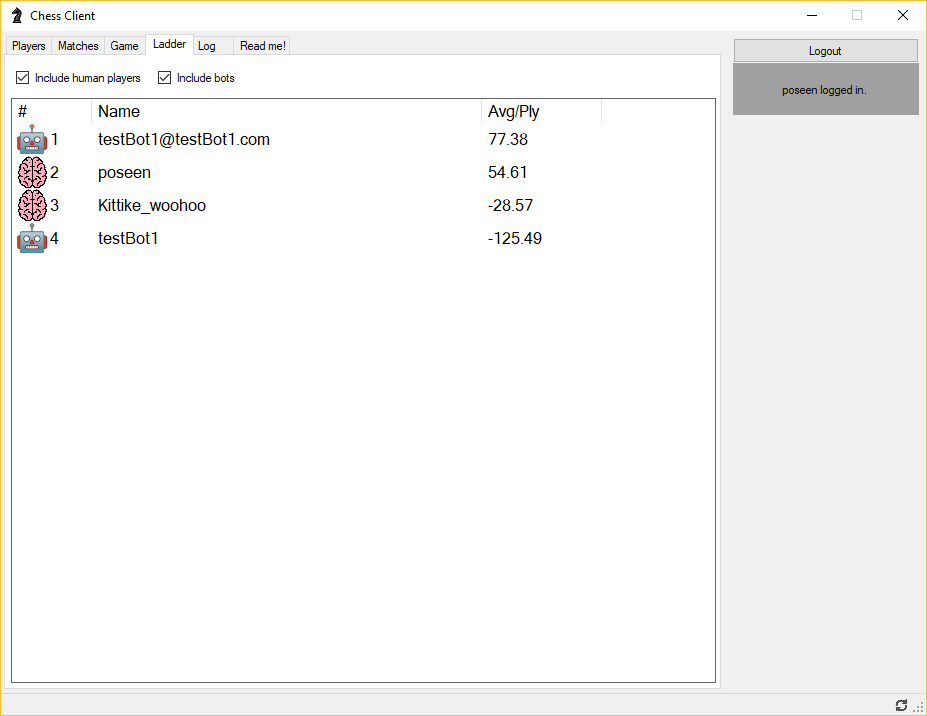
\includegraphics[width=\textwidth]{img/humanClientLadder.png}
		\caption{Toplista}
		\label{fig:humanClientLadder}
	\end{subfigure}
	
	\caption[ Játékkliens UI terv ]
	{\small Játékkliens UI terv}
	\label{fig:humanClient}
\end{figure*}

A különböző funkciók között tabokkal legyen lehetőség lépkedni, bármely felületről bármelyikre át lehessen így kattintani. A "Game" tabon lehessen a kiválasztott játékra válaszolni. Először a mozgatni kívánt bábura, majd az új pozíciójára kattintva kell, hogy elküldje a kliens a kérést a szerver felé-

\subsection{A botkliens felhasználóit felülete}
(Lásd: \ref{fig:botClient})

\begin{figure*}
	\centering
	\begin{subfigure}[b]{0.475\textwidth}
		\centering
		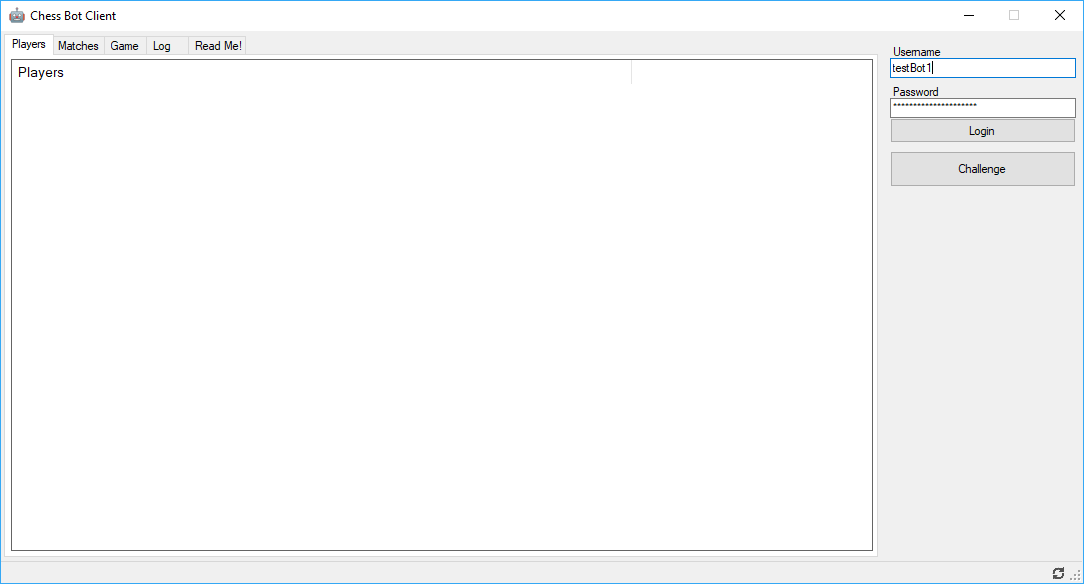
\includegraphics[width=\textwidth]{img/botClientLogin.png}
		\caption{Belépő képernyő}
		\label{botClientLogin}
	\end{subfigure}
	\hfill
	\begin{subfigure}[b]{0.475\textwidth}  
		\centering 
		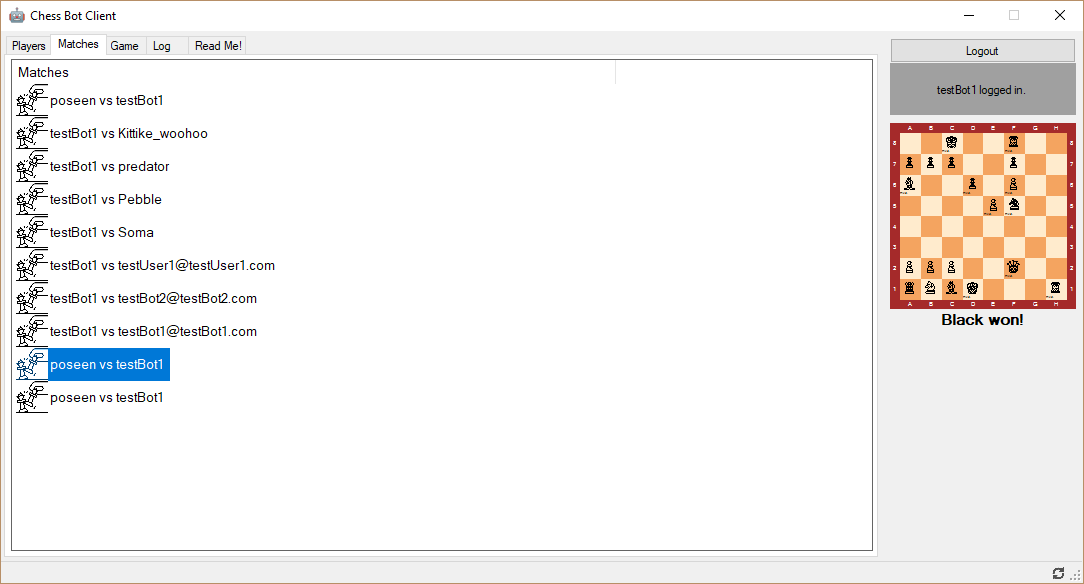
\includegraphics[width=\textwidth]{img/botClientMatches.png}
		\caption{Partik}
		\label{fig:botClientMatches}
	\end{subfigure}
	\vskip\baselineskip
	\begin{subfigure}[b]{0.475\textwidth}   
		\centering 
		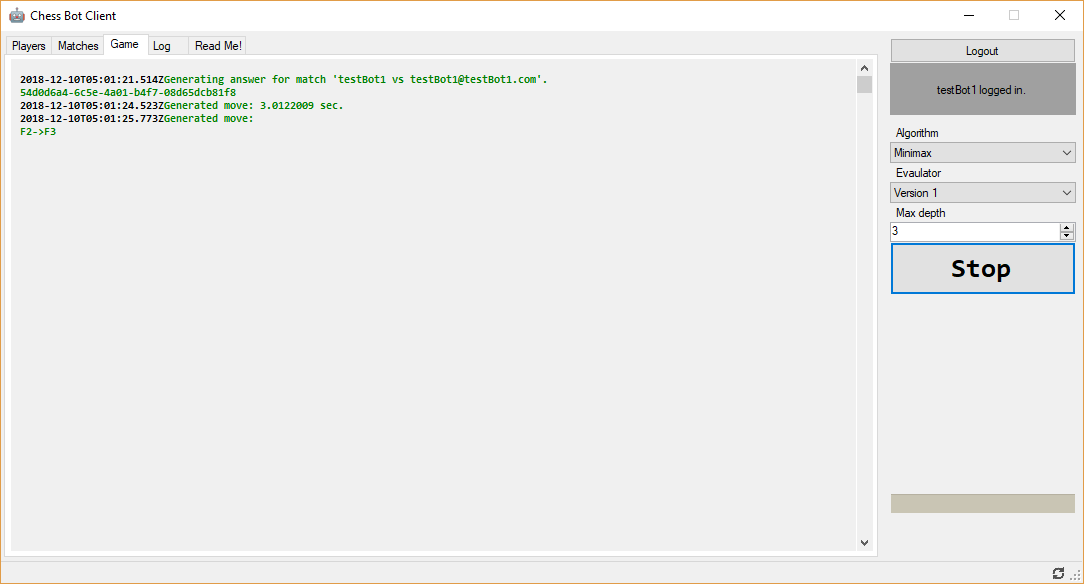
\includegraphics[width=\textwidth]{img/botClientGame.png}
		\caption{Bot vezérlése}
		\label{fig:botClientGame}
	\end{subfigure}
	\quad
	\begin{subfigure}[b]{0.475\textwidth}   
		\centering 
		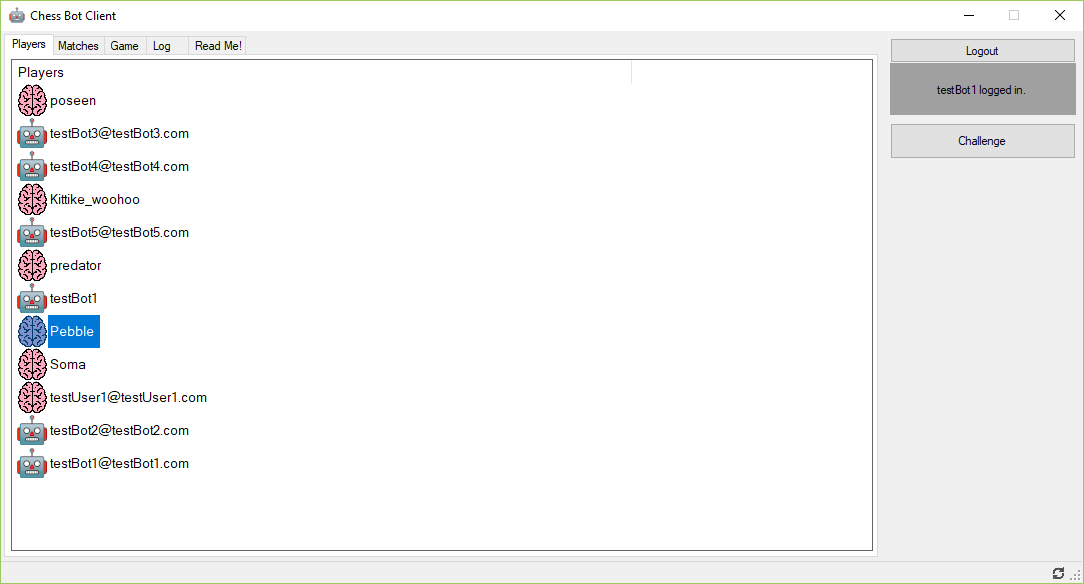
\includegraphics[width=\textwidth]{img/botClientPlayers.png}
		\caption{Játékosok listája}
		\label{fig:botClientPlayers}
	\end{subfigure}
	\caption[ Botkliens UI terv ]
	{\small Botkliens UI terv}
	\label{fig:botClient}
\end{figure*}

A botkliens "Game" tabján lehet vezérelni a botot. A jobb oldalon lehessen kiválasztani az algoritmust, a kiértékelő függvényt, az algoritmus maximális mélységét, illetve ott lehet elindítani és leállítani. A tér nagy részét egy szövegmező foglalja el, ott látszódik, hogy épp mit csinál a bot.

\section{Kommunikáció a szerver és a kliensek között}
A kommunikációról egy sematikus rajz a \ref{fig:clientServerCommunication} ábrán látható.

\begin{figure}[htbp]
	\centering
	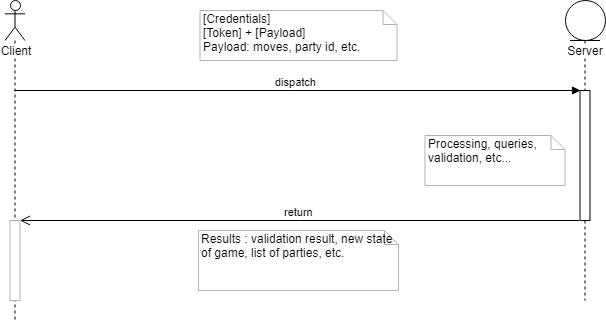
\includegraphics[width=1.0\textwidth]{img/clientServerCommunication.png}
	\caption{Kliens - szerver közötti kommunikáció sémája}
	\label{fig:clientServerCommunication}
\end{figure}

Kérés-válasz séma: a szerver nem küld magától semmilyen információt, nem tart fent a klienssel kapcsolatot, és a szervernek nem is kell semmilyen információt tárolnia az aktuális munkamenetről. Minden kérés önmagában értelmezhetőnek kell lennie és a szervernek minden kérésnél minden információnak rendelkezésre kell állnia ahhoz, hogy válaszolni tudjon. Megfordítva: a kliensnek minden kérést úgy kell összeállítania, hogy a szervernek elegendő információja legyen a válaszadáshoz.

\section{Fejlesztése segítő segédkönyvtárak}
\subsection{A szolgáltatás igénybevételét segítő könyvtár}
A kérések összeállítására tanácsos egy könyvtár implementálása, amire a botokat vagy klienseket író fejlesztők támaszkodhatnak. Ez azért is lehet segítség, hiszen ha a szerverből kijön egy újabb verzió új vagy módosított funkciókkal, akkor egy központi helyről beszerezve ezen könyvtárakat könnyen át tudnak állni az új verzióra.

\subsubsection{Kéréseket összállító könyvtár}
Kell egy olyan könyvtár, amely viszonylag közel áll a szerverhez. Összeállítja a kéréseket, elküldi, fogadja a válaszokat és átalakítja a megfelelő modellre, amellyel a klienst fejlesztő programozó már könnyen tud dolgozni.

\subsubsection{Munkamenetet kezelő könyvtár}
A további könnyítés érdekében a kéréseket összeállító könyvtárra építve érdemes egy munkamenetet kezelő könyvtár létrehozása is. Ez nem azonos az előzőekben emlegetett munkamenettel. E könyvtár feladata az lenne, hogy a kliens fejlesztője elől elrejtse az elosztott rendszerek minden problémáját (szinkronizációs problémák például) és adjon egy olyan felületet, amely kívülről statikusnak néz ki, ám mindig friss információval rendelkezik az aktuális játékról és játékos "munkamenetéről".

\section{A játék-modell és mechanika}
\subsection{Egy körökreosztott általános táblás játék}
Egy körökreosztott általános táblás játék a következő elemekből áll:

\begin{itemize}
	\item \textbf{Modell} \\
	A játékállás ábrázolása sokrétű lehet. Tárolni kell a játékosok listáját, az aktuális játékost és a játéknak megfelelő állást: táblán lévő bábuk vagy asztalon levő kártyák.
	
	\item \textbf{Szabályok} (avagy játékmechanika) \\
	A szabályok határozzák meg, hogy milyen helyzetben mik a lehetséges lépések. Az ezt kiszolgáló osztály legyen a játékmester, aki hozzányúlhat a reprezentációhoz, így biztosítva, hogy a játék mindig a szabályoknak megfelelően menjen.
\end{itemize}

Egy játékot meghatározza a \textbf{kezdőállapota} és az állapotok közötti lehetséges \textbf{állapotátmenetek}. Egy állapot akkor érvényes, ha a kezdőállapotból bármilyen úton eljuthatunk a megadott állapotba. Ezután már adódik az ötlet: egy játékmenetet reprezentálhatunk egy \textbf{\textit{cimkézett}, irányított gráffal}, ahol a csomópontok a lehetséges állapotok, az élek pedig az átmenetek.

\subsection{A sakk-modell}
A sakk modellezésénél két fontos dolgot kell figyelembe venni:
\begin{itemize}
	\item \textbf{A sakktábla problémája} \\
	A sakktábla információhiánya (\ref{A Sakktábla információhiánya}) résznél már értekeztünk arról, hogy nem elég "ránézni" a sakktáblára, további adatok is szükségesek a lehetséges lépések meghatározásához.
	
	\item \textbf{Továbbfejleszthetőség} \\
	Sakktáblán sokféle játékot lehet játszani, de még akkor is sok opciónk van, ha ragaszkodunk a táblához és a sakkbábukhoz. Például ilyenkor lehet beszélni \textit{francia sakkról} vagy a \textit{véletlen-sakkról}, ami ugyanúgy működik, mint a normál sakk, azzal a különbséggel, hogy a kezdőpozíciói a bábuknak véletlenszerű.
\end{itemize}

Ebből két dolog látszik: az egyik az, hogy a játszma aktuális állapotának modelljét el kell választani a szabályoktól, hiszen ugyanazokkal a bábukkal más játékot is lehet játszani.

A másik dolog pedig az, hogy nem elég a táblán lévő bábukra hagyatkozni, be kell vezetni később jelzéseket a bábukra, illetve az eddigi lépéseket is tárolni kell. Így látszik, hogy a játék-modell két komponensből kell, hogy álljon: a \textbf{modellből} és a modell konzisztenciáját fenntartó \textbf{játékmechanikára}, amely kizárólagos módon módosíthatja a modellt a sakk szabályai alapján.

Ebből kell kialakulnia majd egy könyvtárnak, amely a sakkot modellezi és a sakkjátszmákat vezeti le.

\section{Mesterséges intelligencia algoritmusok}
\subsection{A probléma komplexitása}
Fogalmazzuk meg a problémát: szeretnénk egy olyan programot, amely legyőzi a másik játékost (vagy legalábbis nem veszít), ami ekvivalens azzal, hogy minden egyes lépésnél a legoptimálisabb lépést választja.

\textit{Tekintsük egy sakkjátszmát: egy átlagos meccs 35-40 fordulós~\cite{averageLengthOfChessGame}\cite{averageLengthOfChessGame2}\cite{chessStatistics}, az átlagos lehetséges lépések száma egy adott állapotból 20\cite{shannonnumber}. Shannon adott egy alsó-korlátot a lehetséges játékok számára, amely $10^{120}$. \footnote{Összehasonlításképp: a világegyetemben levő atomok számát $10^{80}$ darabra teszik, a világegyetem pedig körülbelül $4.32 \times 10^{17}$ másodperce keletkezett, ami kevesebb, mint $10^{18}$-on, ami még így is sok nagyságrenddel kevesebb, mint a lehetséges játékok száma.} Ebből látható, hogy \textit{brute-force} technikával, a jelenlegi technikai háttérrel nem érdemes hozzákezdeni.}

Így a probléma elég bonyolult és ezért egzakt megoldása nem létezik egyelőre, csak közelíteni tudjuk. A továbbiakban az algoritmust általánosan fogalmazzuk meg és formalizáljuk, de a sakkon keresztüli példákon mutatjuk be.

\subsection{A probléma, mint útkeresési algoritmus}
Láthatjuk, hogy így egy játékmenet az irányított gráf egy útja lesz. A probléma pedig amit az algoritmussal meg szeretnénk oldani (vagy közelíteni) pedig az, hogy találjunk egy olyan útvonalat ebben a gráfban, amelyben a nyereségünket maximalizálni, vagy legalább az ellenfél nyereségét minimalizálni próbáljuk.

A sakk nem más, mint egy körökre osztott két személyes táblás játék és a fenti analógia alkalmazható rá: Kezdetben van egy kezdőállapot. (Felállított bábuk a táblán, világos játékos kijelölve mint kezdőjátékos). Ezek után az állapotátmeneti függvény határozza meg a lehetséges lépések halmazát, amelyből egy irányt kiválasztva és követve egy új állapotba kerülünk, és így tovább. Ez lesz a játék \textbf{játékgráfja}.

\subsection{Egy általános gráf. Fa-e vagy sem?}
Erről a gráfról semmi érdemlegeset nem állíthatunk, nem speciális, hiszen előfordulhat, hogy más utakon is eljuthatunk ugyanazon csúcsba, tehát nagy valószínűség szerint nem fa. Ezt a problémát megszüntethetjük többféle módon, például: 

\begin{itemize}
	\item \textbf{Csomópont duplázással} \\
	Ilyenkor az történik, hogy ha egy állapotba több úton is eljuthatunk, akkor ezeket a csúcsokat többszörözzük. \\
	(Lásd.: \ref{fig:game-graph-transformation} ábra.)
	
	\item \textbf{Ügyes reprezentációval} \\
	Ilyenkor azt tesszük, hogy elgondolkodunk: attól, hogy ugyanabba a csomópontba jutunk több úton, az nem jelenti-e esetleg azt, hogy a más úton elért csúcs már inkább egy másik csúcs. Sakkos példánál maradva: ezt úgy érhetjük el, hogy egy állapot reprezentációjába bevesszük az odavezető utakat. Például előállhat egy hasonló állapot, ha mi is és az ellenfél is előrelép majd vissza ugyanazzal a bábuval.
\end{itemize}

\begin{figure}[htbp]
	\centering
	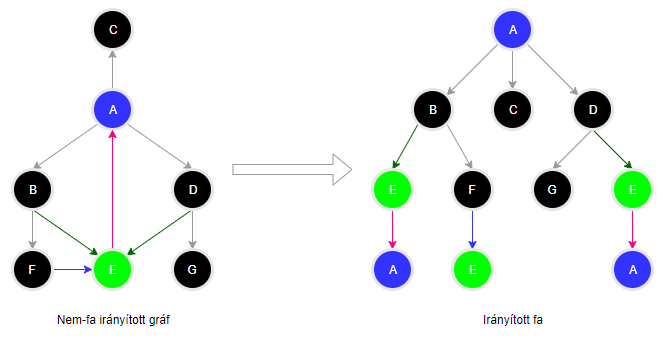
\includegraphics[width=1.0\textwidth]{img/game-graph-transformation.png}
	\caption{Általános irányított gráfból irányított fa konstruálása}
	\label{fig:game-graph-transformation}
\end{figure}

\subsection{Nem is kell feltétlenül fa}
Tegyük fel, hogy van egy algoritmusunk, amely kiszámítja a saját és az ellenfél legmegfelelőbb lépéseit a játék végéig. Így megkapjuk az utat ami a mi győzelmünkhöz vagy legalább az éppen legjobb elérhető eredményhez vezet. Ez nem feltétlen célravezető, hiszen mi történik akkor, ha az ellenfél végül nem azt a lépést lépi valamilyen okból? (Lehet, hogy az ő algoritmusa jobb vagy rosszabb, mint a mienk. Lehet, hogy más kiértékelőfüggvényt használ, stb.) Ekkor azt látjuk, hogy a sok munka, amellyel felépítettük az utat, kárba vész. Ezért nem érdemes az egész utat felépíteni, elég csak annyit elvárni tőle, hogy adjon egy javaslatot a következő lépésre. Természetesen a "hogyan" kérdésre a válasz lehet elég bonyolult is (minimax-, alfa-béta-, genetikus- és tanuló-algoritmusok trükkös heurisztikákkal), de a vége ugyanaz: egy lehetőleg legoptimálisabb lépés kiszámítása. Mivel nem fogjuk bejárni az egész fát csak egy adott mélységig, ezért a lépések száma véges lesz, így már nem probléma ha a gráf nem fa (azaz van benne kör), így a probléma nem is biztos, hogy létezik.

\subsection{Mesterséges Intelligencia Algoritmusok könyvtára}
Érdemes definiálni egy mesterséges intelligencia általános algoritmusokat megvalósító könyvtárat is, ezzel nyújtva további segítséget a jövőbeli fejlesztőknek. Ez azért is hasznos, mert az algoritmusok nem változnak, a nagy különbség a játékállapotot kiértékelő implementációban van, így elég, ha a programozó arra koncentrál.

\section{Összefoglalás}
Ezek alapján összegezzük a leendő programcsomag szerkezetét és különböző elemeinek feladatát:

\begin{itemize}
	
	\item \textbf{Játék-modell} (könyvtár)
	\begin{itemize}
		\item Megvalósítja a játéktér modelljét
		\item Ezen játéktérhez megvalósítja a sakk szabályait
	\end{itemize}
	
	\item \textbf{Algoritmusok} (könyvtár)
	\begin{itemize}
		\item Definiál egy interface-t
		\item Tartalmazza néhány algoritmus általános megvalósítását:
		\begin{itemize}
			\item Minimax, átlagoló minimax
			\item Alfa-béta
			\item Egyéb egyszerűbb példák teszteléshez (random, mohó)
		\end{itemize}
		\item Könnyen használható és kiterjeszthető más alkalmazásokban.
	\end{itemize}
	
	\item \textbf{Architektúra}
	\begin{itemize}
		\item \textbf{Szerver}
		\begin{itemize}
			\item Felhasználó regisztrációja / hitelesítése / nyomonkövetése.
			\item Ellenőrzi a kliensektől jövő lépések érvényességét.
			\item Közvetíti a kliensek felé a partik alakulását.
		\end{itemize}
		
		\item \textbf{Kliens (humán vagy MI kliens)}
		\begin{itemize}
			\item Felhasználó beléptetése, nyomonkövetése.
			\item Közvetíti a felhasználó felé a partik alakulását.
			\item A játékos döntéseit közvetíti a szerver felé.
			\item Példakliensek implementálása:
			\begin{itemize}
				\item Játékkliens
				\item Botkliens
			\end{itemize}
		\end{itemize}
	\item \textbf{Kliens-közeli könyvtárak}
	\begin{itemize}
		\item \textbf{Szerverközeli klienskönyvtár}
		\begin{itemize}
			\item Könnyen kezelhető interfészt ad
			\item Összeállítja a kéréseket
			\item Visszajövő válaszokat a kliensfejlesztő számára könnyen feldolgozható modellé alakítja
		\end{itemize}
		\item \textbf{Játék munkamenet-könyvtár}
		\begin{itemize}
			\item Egy egyszerű interface-t ad
			\item A szerverközeli klienskönyvtárra épül
			\item Szinkronizációs feladata van
			\item "Business object"-ként funkcionál
		\end{itemize}
	\end{itemize}
	\end{itemize}
\end{itemize}

\newpage
\chapter{Megvalósítás}
\noindent A projekt fontosabb részeinek felépítését lásd: \ref{fig:solutionStructure}. ábra.

\begin{figure}[htbp]
	\centering
	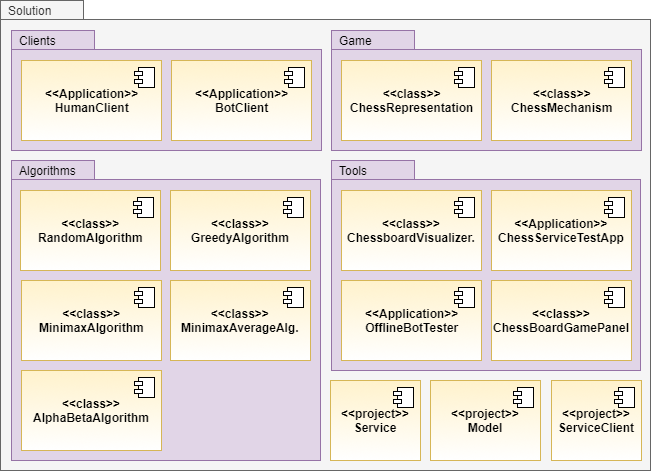
\includegraphics[width=1.0\textwidth]{img/solutionStructure.png}
	\caption{AlphaBetaAlgorithm osztály}
	\label{fig:solutionStructure}
\end{figure}

\section{A sakk megvalósítása (\texttt{Game} projekt)}
\subsection{Egy általános körökreosztott táblás játék modellje}
Kezdjük megint egy általános megközelítéssel: Legyen \texttt{GameModel} osztály, ami reprezentálja egy játék egy állapotát. Csak tárolja a tábla vagy asztal aktuális állapotát és lehetőséget biztosít a módosítására. Nem szabad semmilyen játék alapelveit beleépíteni, hiszen például egy sakktáblán is lehet többfajta sakkot játszani, amelyek szabályai különbözőek.

A \texttt{GameMechanism} osztály a "játékmester", ő az, aki a szabályok szerint módosítja a reprezentációt. Rajta keresztül kell validálni és végrehajtatni a lépéseket, illetve tőle lehet lekérdezni az aktuális meccs állását illetve egyéb fontosabb tulajdonságait. 

Egy a fentieknek megfelelő magasszintű terv látható a \ref{fig:boardGameAbstractClassDiagram}. ábrán.

\begin{figure}[htbp]
	\centering
	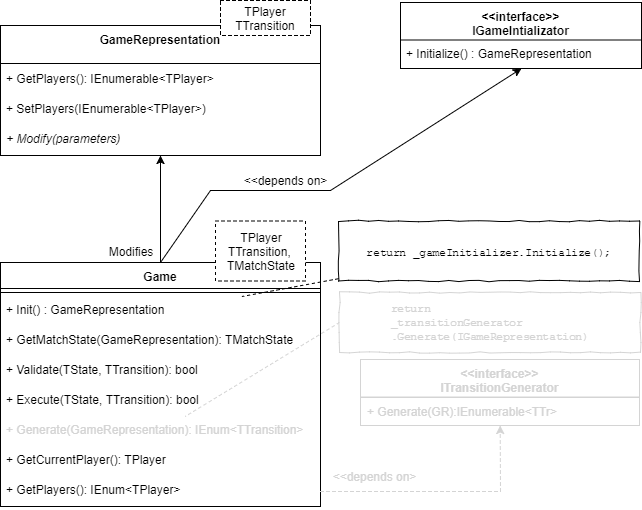
\includegraphics[width=1.0\textwidth]{img/boardGameAbstractClassDiagram.png}
	\caption{Egy általános táblás, körökre osztott játék absztrakt reprezentációja}
	\label{fig:boardGameAbstractClassDiagram}
\end{figure}

\subsection{A modell (\texttt{ChessRepresentation} osztály)}
Az előző fejezetekben végiggondoltuk, hogy mi a minimális információmennyiség, amely ahhoz kell, hogy egy sakkjátszma egy állapotát leírjuk úgy, hogy abból egyértelműen kiszámítható legyen a lehetséges lépések halmaza. Ezek alapján sejthető a lehetséges reprezentáció: egy sakk-állás leírásához a következő információk kellenek:
\begin{itemize}
	\item Tábla állapota
	\item Következő játékos
	\item Bábuk jelölése (elmozdult? en passant?)
	\item Eddig megtett lépések listája
\end{itemize}

Illetve az előzőekben megtárgyaltuk, hogy hogyan is lehet érdemes modellezni és implementálni a sakkot, ha a későbbiekben továbbfejlesztési terveink vannak vele: A sakk is két fő részből áll: modell és játékmechanika. Ezeket a \texttt{ChessBoard} és a \texttt{ChessGame} osztályok valósítják meg. (Lásd: \ref{fig:chessClassDiagram}. ábra.)

\begin{figure}[htbp]
	\centering
	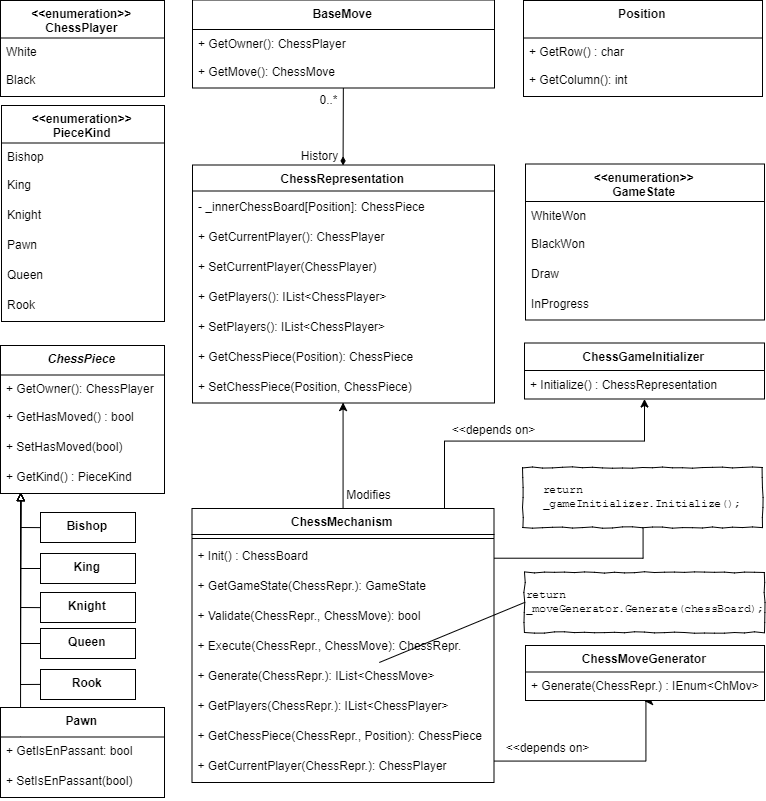
\includegraphics[width=\textwidth]{img/chessClassDiagram.png}
	\caption{Sakkot reprezentáló osztálydiagram}
	\label{fig:chessClassDiagram}
\end{figure}

\textit{A \texttt{Generate()} függvény azért van kiszürkítve az ábrán, mert egy játék lehetséges lépései nem feltétlen diszkrét értékek egy véges halmaza. Szigorúan véve csak azt kell megkövetelni a \texttt{GameMechanism} osztálytól, hogy el tudja dönteni egy bejövő lépésről, hogy az érvényes-e. A lépések kigenerálása inkább csak a mesterséges intelligencia algoritmusának "jöhetne jól".}

A sakktáblát reprezentáló \texttt{ChessBoard} osztály az előzőekben részletezett alapelveknek felel meg. Legfontosabb művelete a \texttt{Move(from, to)} függvény, amely elvégzi a módosításokat a táblán, ám a \texttt{History}-ba nem írja be, az majd a "játékmester" feladata lesz. Továbbá a \texttt{Move()} függvény visszatérési értéke a "leütött" bábu, vagy \texttt{null} ha üres volt.

A sakktáblát egy egydimenziós tömb tárolja, amin a tájékozódás kissé nehézkés, ezért a sakkhoz jobban illő \texttt{Position} tipuson keresztül lesz ez megkönnyítve, amely az \textit{algebrai lejegyzést} használja.

A későbbi fejlesztések segítéséhez az osztály tartalmaz konvertereket (array index és pozíció között oda-vissza) és egyenlőségvizsgálatot is, hogy írhassuk: \texttt{p1 == p2} vagy \texttt{p1.Equals(p2)}.

Ezeken kívül - kissé lazábban kapcsolódva a szigorúan vett feladathoz - implementálva lett a \texttt{Position} osztályhoz néhány kiterjesztés is, amely a sokszor használt pozícióval kapcsolatos műveleteket implementálja. Ilyen például az "északi irányba lépés" vagy a "lólépés", illetve a diagonális, horizontális és vertikális lépések listájának kigenerálása. Ezt valósítja meg a \texttt{PositionExtensions} osztály (Lásd \ref{lst:chessboardpositionextensions_code}. kódrészlet).

\begin{lstlisting}[caption=Pozíciók segédfüggvényes - PositionExtensions osztály, label=lst:chessboardpositionextensions_code, float,floatplacement=H]]
public static class PositionExtensions
{
	public static Position ParsePostal(this string postalNotation) { /* ... */ }

	public static Position North(this Position position, int number = 1) { /* ... */ }
	public static Position South(this Position position, int number = 1) { /* ... */ }
	public static Position West(this Position position, int number = 1) { /* ... */ }
	public static Position East(this Position position, int number = 1) { /* ... */ }
	public static Position NorthEast(this Position position, int number = 1) { /* ... */ }
	
	/* ... */

	public static Position KnightNorthEast(this Position position)
	{
		var newPosition = position.North(2).East(1);
		return newPosition;
	}

	public static Position KnightNorthWest(this Position position) { /* ... */ }

	/* ... */

	public static IEnumerable<Position> KnightMoves(this Position position)
	{
		var possibleMoves = new []
		{
			position.KnightSouthWest(),
			position.KnightSouthEast(),
			position.KnightWestSouth(),
			position.KnightWestNorth(),
			position.KnightEastSouth(),
			position.KnightEastNorth(),
			position.KnightNorthWest(),
			position.KnightNorthEast()
		}.Where(x => x != null);
		
		return possibleMoves;
	}

	public static IEnumerable<Position> Northwards(this Position position, int maxRadius = int.MaxValue) { /* ... */ }

	/* ... */

	public static IEnumerable<Position> StraightMoves(this Position position, int maxRadius = int.MaxValue) { /* ... */ }
	public static IEnumerable<Position> DiagonalMoves(this Position position, int maxRadius = int.MaxValue) { /* ... */ }
	public static IEnumerable<Position> AllDirectionsMove(this Position position, int maxRadius = int.MaxValue) { /* ... */ }
}
\end{lstlisting}

A kiterjesztési függvények segítségével szép láncolt kifejezéseket lehet szerkeszteni, példa erre a \texttt{KnightNorthEast} függvény, ahol könnyen leolvasható miből is áll egy észak-keleti irányba lépő huszár: "kettőt északra, egyet keletre".

\subsection{A sakk-mechanizmus (\texttt{ChessMechanism} osztály)}

A sakk implementációja sokkal bonyolultabb és felvet néhány érdekes problémát. Minden függvény első bemenő paramétere egy modell. Ebből állapítja meg, hogy mik a lehetséges lépések (\texttt{GenerateMoves}), egy megadott lépés helyes-e az adott helyzetben (\texttt{ValidateMove}) és alkalmazza a megadott lépést ha helyes (\texttt{ApplyMove}). Ezeket külön-külön megvizsgáljuk:

\subsubsection{GenerateMoves()}
A \texttt{GenerateMoves} függvény az egész osztály legfontosabb függvénye. Erre építkezik több másik függvény is. Mivel minden állapotban a lehetséges lépések halmaza véges és diszkrét, ezért implementálható és felhasználható más függvényekben is. \textit{(Ha nem lenne implementálható, akkor csak a \texttt{ValidateMove} és az \texttt{ApplyMove} függvényeket lehetne implementálni.)}

A lépések kigenerálásának két lépése van: a naív kigenerálás és az illegális lépések kiszűrése.
\begin{enumerate}
	\item \textbf{Lehetséges lépések naív kigenerálása}
	\begin{itemize}
		\item \textbf{Normál lépések kigenerálása} \\
		A legtöbb báb ahová léphet, ott üthet is. Így ezen lépések kigenerálása egyszerű, csupán annyi megszorítással például egy futónál, hogy habár bármennyit léphet diagonálisan, bábut nem ugorhat át, így a saját bábu esetében előtte meg kell állnia, vagy ellenfél bábuja esetében azt leütve a helyére kell lépnie és tovább nem mehet.
		
		\item \textbf{A gyalog lépései} \\
		A gyalog lépéseinek kigenerálása az egyik bonyolult függvény. Eleve ketté kell osztani a lépéseit, ugyanis neki vannak olyan lépései, amelyek nem ütnek. A gyalog csak "srégen előre" tud ütni, viszont lépni (ha van helye) előre is tud. Ezért ezt a két esetet szét kell választani, amely majd jól jön később, amikor a sakkba lépést vizsgáljuk. 
		
		\item \textbf{Sáncolás} \\
		A sáncolásnak több előfeltétele is van: a benne résztvevő bástya és a király nem mozdulhatott még el a parti alatt, a király nem lehet támadva ("sakkban"), illetve a király által lépdelt mezők sem lehetnek támadva. Ez így elég sok feltétel, ráadásul rendhagyó is. Az előzőekben részletezett lépéseknél könnyen használható a későbbi szűrés, de mivel itt szigorúan véve nem csak egy lépés, hanem egy lépéssorozat történik és minden lépésben meg kell vizsgálni, hogy támadva van-e a sáncolás útvonala, ezért ezt "helyben" kell elvégezni. Ehhez ki kell számolni azokat a mezőket, amelyek támadás alatt vannak. (Ez egy érdekes rekurzív problémához vezet.)
	\end{itemize}
	
	\item \textbf{Szabályokkal ellenkező lépések kiszűrése} \\
	Meg kell vizsgálni, hogy az adott lépés "felfedi-e" a királyt egy támadó bábunak. Ez esetben a lépés nem lehetséges. Ezt úgy tudjuk megvizsgálni, hogy kiszámoljuk a saját lépésünk utáni támadott mezőket és megnézzük, hogy ezek között szerepel-e a király pozíciója. Ugyanez az eljárás sakk esetén is, hiszen ez esetben pedig csak olyan lépések jöhetnek számításba, amelyek megszüntetik a sakkot. Ha ilyen lépés nem létezik, akkor megtörtént a sakk-matt.
	
	A szűrésnél a másik dolog amire figyelni kell, hogy csak a támadó lépéseket kell figyelembe venni. Ez a gyalog lépéseinél jöhet szóba, hiszen egy gyalog léphet előre, ám ott nem üthet, ezért a király például léphet az ellenfél gyalogja elé. Ezért is kell szétválasztani a gyalog esetében a normál- és ütőlépések kigenerálását.
\end{enumerate}

\paragraph{\textit{Egy érdekes rekurziós probléma}} \mbox{} \\
\textit{A sáncolás kiszámításánál futhatunk bele egy trükkös rekurzióba. A feltételek ellenőrzésének része, hogy megállapítsuk: a megfelelő mezők és bábuk támadva vannak-e. Ehhez meg kell állapítani az éppen az ellenfél által veszélyeztetett mezőket. Ehhez ki kell generálnunk az aktuális helyzettől függő ellenfél lépéseit, amelynek viszont része a sáncolás is. Így egy végtelen rekurzióhoz jutunk. Ezt úgy lehet megszüntetni, hogy a veszélyeztetett mezők kiszámításánál nem vesszük figyelembe az ellenfél sáncolását, hiszen az semmilyen esetben nem lehet hatással a mi sáncolásunkra.}

\subsubsection{ValidateMove()} \mbox{}
Ennél a játéknál szerencsénk van: ha a \texttt{GenerateMoves()} függvény implementálható (azaz a következő lehetséges lépések halmaza véges és diszkrét elemekből áll) akkor nincs más dolgunk, mint megállapítani: a beérkezett lépés benne van-e a kigenerált lehetséges lépések között.

\subsubsection{GetGameState()}
A \texttt{GetGameState} függvény hivatott kiszámolni, hogy mi a játék aktuális állapota? Ha van még lehetséges normál lépés, akkor jelzi, hogy lehet még lépni, ha bármilyen módon vége van (valaki feladta, mattot adott vagy patt-helyzet alakult ki) akkor azt jelzi. Ehhez az utolsó lépést vizsgálva és a \texttt{GenerateMoves} függvényt meghívva számolja ki a kimenetet:

\begin{itemize}
	\item Ha az utolsó lépés egy döntetlen elfogadása $\to$ döntetlen.
	\item Ha az utolsó lépés egy feladás $\to$ ellenfél játékosa nyert.
	\item Ha van még lépés $\to$ A játék folyamatban van.
	\item Ha nincs már lépés, akkor...
	\begin{itemize}
		\item Ha az aktuális játékos sakkban áll $\to$ MATT
		\item Ha az aktuális játékos nem áll sakkban $\to$ PATT (döntetlen)
	\end{itemize}
\end{itemize}

\subsubsection{ApplyMove()}
Az \texttt{ApplyMove} függvény végrehajtja a megfelelő módosításokat a táblán és a lépést "lejegyzi". Kimenete a módosítás utáni reprezentáció. Ha a lépés nem megengedett \texttt{null}-lal tér vissza.

\section{MI algoritmusok (\texttt{Algorithms} projekt)}
\subsection{Algoritmusok absztakt interface-e}
Az algoritmusok interfésze nem bonyolult: egyetlen függvénye van, a \texttt{TMove Calculate(TState state)}, amely paraméterként kap egy aktuális állapotot (játék-modellt) és visszatér egy lépéssel. (Lásd: \ref{fig:algorithmAbstractDiagram}. ábra.)

\begin{figure}[htbp]
	\centering
	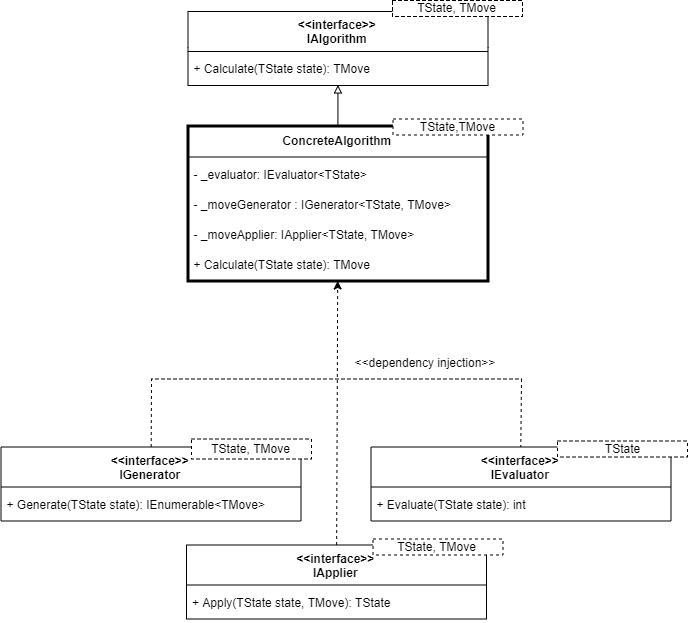
\includegraphics[width=0.7\textwidth]{img/algorithmAbstractDiagram.png}
	\caption{Absztrakt algoritmus interface és függőségei}
	\label{fig:algorithmAbstractDiagram}
\end{figure}

A konkrét megvalósításhoz kellhet egy kis segítség. Az algoritmusnak sok lehetséges lépésből kell kiválasztania a legmegfelelőbbet. Ehhez három dolog kell:

\begin{itemize}
	\item \textbf{Lépés-generátor} \\
	Segédkezik a lehetséges lépések kigenerálásában.
	
	\item \textbf{Kiértékelő} \\
	A kiértékelő osztály mondja meg egy állapotról, hogy az "mennyire jó".

	\item \textbf{Alkalmazó} \\
	Ez az osztály hivatott módosítani a reprezentációt, valójában egy "wrapper" osztály a valódi "játékmester osztályhoz".
\end{itemize}

\subsubsection{A generátor interface} Az algoritmus nem tud semmit a sakkról és nem is kell neki. Azt, hogy milyen lépések lehetségesek, kívülről megadott függőségek fogják megadni. Így a megvalósítás lehet a játékhoz készült generátor osztály köré rakott wrapper vagy proxy-osztály, de lehet több felelőssége is. Egyetlen függvénnyel rendelkezik, egy megadott állapotra alkalmazva visszaadja a lehetséges lépések (egy) halmazát. Lehet egyszerű és elég bonyolult is. A következő lépéseket tartalmazhatja:

Első lépésben diszkretizálhat: például ha a játék lehetséges lépéseinek száma egy adott állapotban végtelen, ekkor véges számú lépéseket gyárt és azt adja vissza. Ha - mint például a sakkban - minden állapotból csak véges sok lépés lehetséges, akkor azokat adja vissza.

Második lépésben szűrhet. Például egy heurisztika alapján az első lépésben megkapott listát leszűrheti az alapján, hogy mit van értelme megvizsgálni és mit nem.

Harmadik lépésben sorrendiséget határozhat meg. Ez például jól jöhet az alfa-béta algoritmusnál, ahol a bejövő lehetséges lépések sorrendjének az eredményre bár nincs hatása, de a futási időre már annál inkább lehet. Ha a lépések pont "rossz sorrendben" jönnek be, akkor az alfa-béte lefutása nem lesz jobb a minimax lefutásánál. Ha viszont "jó sorrendben" jönnek a lépések vizsgálatra, akkor drasztikus sebességnövekedést lehet elérni az alfa-béta algoritmussal. (Egy kedvező és egy kedvezőtlen esetet láthatunk a \ref{fig:alphabeta_examples} ábrán.)

\subsubsection{Az alkalmazó interface} Egyetlen függvénnyel rendelkezik, egy megadott állapotra alkalmazza a megadott lépést és visszaadja az új állapotot. Legtöbbször egy wrapper a játékot kezelő osztály körül.

\subsubsection{A kiértékelő interface}
Kell egy kiértékelő-osztály is, amely eldönti az újonnan előállt állapotról annak értékét az aktuális játékos szemszögéből. Erre jelen esetben az \texttt{integer} megfelelő választás lesz, maximum és minimum értékét (\texttt{int.MaxValue} és \texttt{int.MinValue}) extremális elemként használva. A minimum érték jelentse a $-\infty$-t, a maximum érték pedig jelentse a $+\infty$-t.\footnote{Megjegyzendő, hogy a visszaadott érték nem feltétlen kell, hogy egy sima természetes vagy valós szám legyen, de fontos, hogy az \texttt{TResult Evaulate(TState state)} függvénynek a \texttt{TResult} típusérték-halmazának legalább részben-rendezett halmaznak kell lennie.}
Egyetlen függvénnyel rendelkezik, a megadott állapotra ad egy pontértéket az aktuális játékos szemszögéből.

\subsection{Véletlen-algoritmus (\texttt{RandomAlgorithm} osztály)}
A lehetséges lépések közül véletlenszerűen választ egyet. Működése nagyon egyszerű: nem végez kiértékelést, csak a lehetséges lépések közül választ egyet. Néha szerencséje van.
Használata akkor javasolt, amikor egy gyors algoritmusra van szükségünk egy-egy új koncepció teszteléséhez, vagy a szerver teherbírásának kipróbálásakor sok adat generálásánál.

\subsection{A mohó algoritmus (\texttt{GreedyAlgorithm} osztály)}
A mohó algoritmusban habár már van logika, az nem feltétlen célravezető. A lehetséges lépések közül azt választja, amelyik a legnagyobb veszteséget okozza a következő körben az ellenfél játékosának. A mohó algoritmus nagy hibája, hogy meg fog találni egy lokális maximumot, de nem feltétlen találja meg a globális maximumot. Ezt egyébként onnan is lehet látni, hogy meglepően agresszíven játszik. Ha lehetséges, üt. Ha lehetséges, sakkot ad, és nem érdekli, hogy utána esetleg veszít egy tisztet.
(Példát lásd \ref{fig:greedyAlgorithmExampleDangerous}. ábra.)
\begin{figure}[htbp]
	\centering
	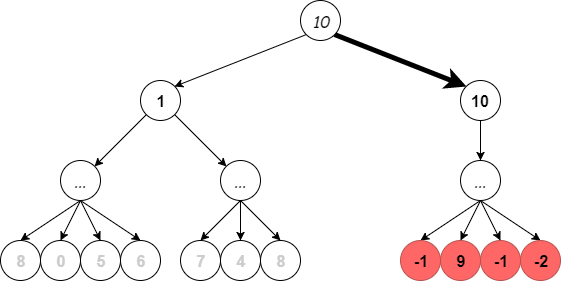
\includegraphics[width=\textwidth]{img/greedyAlgorithmExampleDangerous.png}
	\caption{Mohó algoritmus működése és ahogy tévútra vezet a lokális maximum.}
	\label{fig:greedyAlgorithmExampleDangerous}
\end{figure}

\subsection{A minimax-algoritmus(\texttt{MinimaxAlgorithm} osztály)}
Most nézzük a Minimax algoritmust, mely absztrakt UML diagramja \ref{fig:minimaxAbstractDiagram}. ábrán látható.

\begin{figure}[htbp]
	\centering
	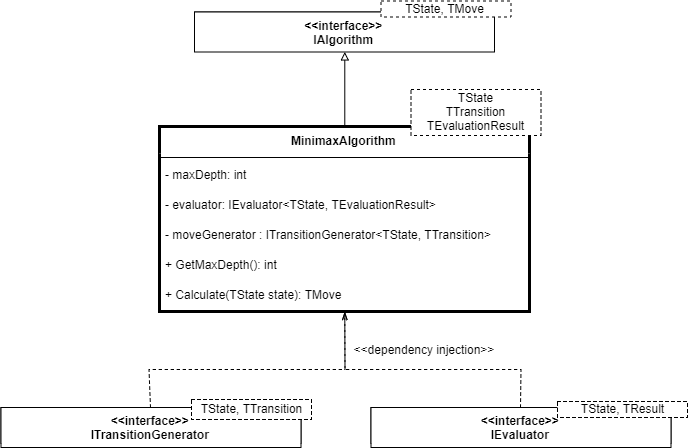
\includegraphics[width=0.7\textwidth]{img/minimaxAbstractDiagram.png}
	\caption{MinimaxAlgorithm osztály}
	\label{fig:minimaxAbstractDiagram}
\end{figure}

A minimax algoritmus lényege, hogy a maximum-mélységben kiértékeli az állásokat, és ezeknek a maximumát illetve minimumát viszi tovább attól függően, hogy melyik szinten van. Első szint a MAX szint, ahol a következő szinten levő csomópontok közül abba az irányba indulunk el, amelyik a legkisebb, ezzel próbálva minimalizálni az ellenfél nyereségét. Következő szint a MIN szint lesz, ahonnan a legnagyobb értékű csomópont felé indulunk el, hogy maximalizáljuk a nyereséget. (Példát lásd \ref{fig:minimaxVsAverageExample}. ábra.)\cite{bevMiHu}
\subsubsection*{Hatékonyság} Tegyük fel, hogy minden csomópontból $x$ a lehetséges lépések száma és $d$ a maximum mélység amit vizsgálunk. Ekkor az algoritmus műveletigénye: $ \mathcal{O}(x^d)$.\cite{alfaBetaPruneHu}

\subsection{Az átlagoló eljárás (\texttt{MinimaxAverageAlgorithm} osztály)}
A minimax algoritmus egy általánosítása. \textit{Avagy a minimax algoritmus az átlagoló eljárás egy speciális esete.} A probléma a statikus kiértékelő-függvényekkel az, hogy lehetetlen olyat megadni, amely megbízhatóan értékeli ki az állásokat. Lehet, hogy egy nagyon jónak ígérkező állásról kiderül, hogy csak egy "csapda" volt és onnan nehezebb vagy lehetetlen megnyerni a meccset. Erre a problémára adhat egy jobb megoldást az átlagoló eljárás. Az ötlet mögötte az, hogy míg az eredeti Minimax algoritmus mindig az aktuális csúcsból elérhető csúcsok minimumát vagy maximumát veszi, addig az átlagoló eljárás a kiterjesztett csúcsok értékeinek MAX szinten az $m$ legnagyobb átlagát, MIN szintjén az $n$ legkisebb átlagát veszi. (Példát lásd \ref{fig:minimaxVsAverageExample}. ábra.)\cite{bevMiHu}

Tehát ha úgy vesszük, akkor a minimax algoritmus nem más, mint az átlagoló-minimax $m=1$ és $n=1$ esetén.

\begin{figure}[htbp]
	\centering
	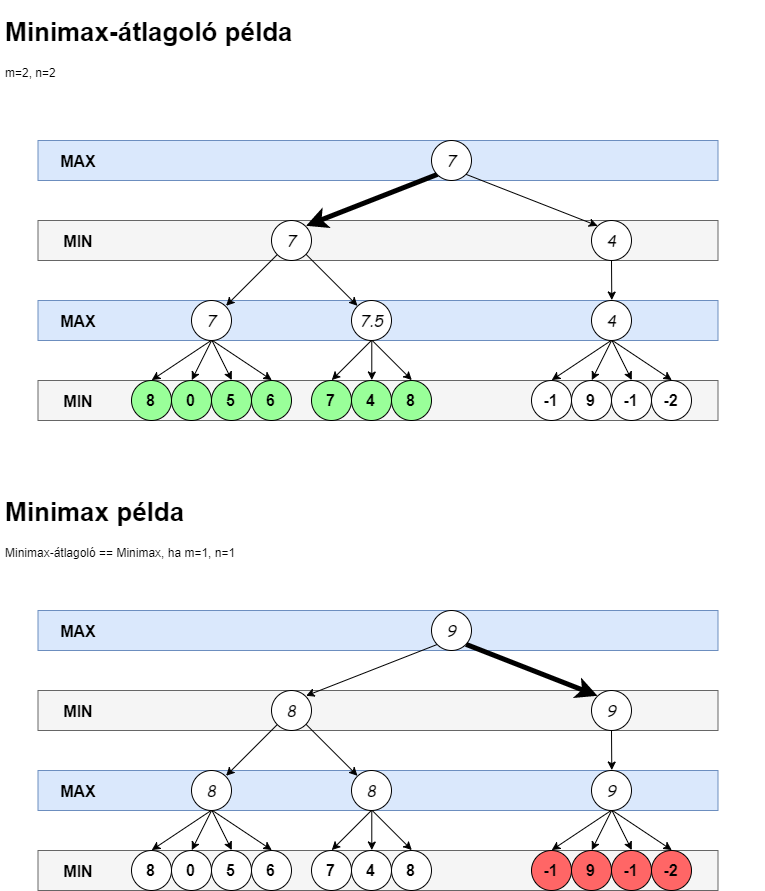
\includegraphics[width=\textwidth]{img/minimaxVsAverageExample.png}
	\caption{Minimax és Átlagoló eljárás összehasonlítása\cite{bevMiHu}}
	\label{fig:minimaxVsAverageExample}
\end{figure}
\subsubsection*{Hatékonyság.} Ugyanaz, mint a minimax algoritmus esetében. Tegyük fel, hogy minden csomópontból $x$ a lehetséges lépések száma és $d$ a maximum mélység amit vizsgálunk. Ekkor az algoritmus műveletigénye: $ \mathcal{O}(x^d)$.\cite{alfaBetaPruneHu}

\subsection{Az alfa-béta algoritmus (\texttt{AlphaBetaAlgorithm} osztály)}
Az alfa-béta algoritmus felépítése nagyon hasonló a minimax-ok felépítéséhez. Absztrakt UML diagramja \ref{fig:alphaBetaAbstractDiagram}. ábrán látható.

\begin{figure}[htbp]
	\centering
	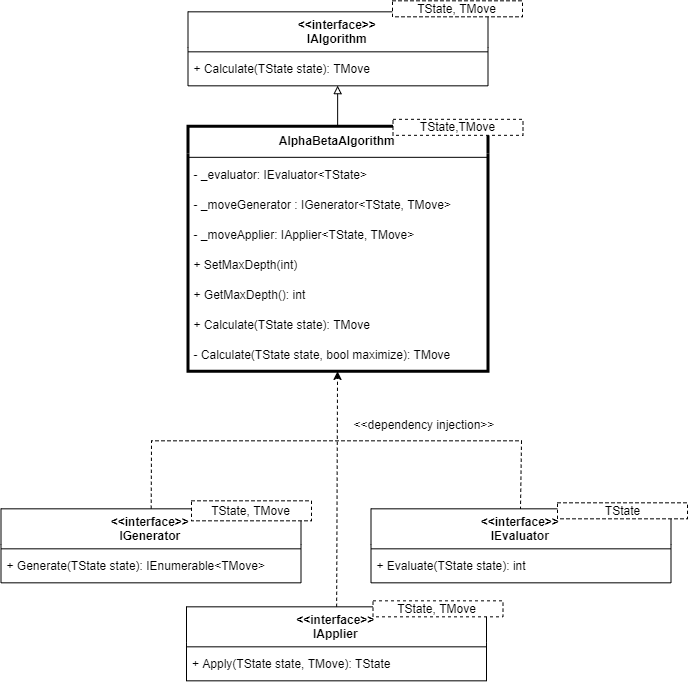
\includegraphics[width=0.7\textwidth]{img/alphabetaAbstractDiagram.png}
	\caption{AlphaBetaAlgorithm osztály}
	\label{fig:alphaBetaAbstractDiagram}
\end{figure}
Az alfa-béta algoritmus a minimax egy továbbgondolása. Megpróbálja levágni azokat az ágakat, amelyeket nem érdemes már vizsgálni. Ez jól jön a számítási-igény csökkentésénél. Az esetek túlnyomó többségében ugyanazt az eredményt kell adnia, mint a minimax-algoritmusnak.

\subsubsection*{Hatékonyság.} Tegyük fel, hogy minden csomópontból $x$ a lehetséges lépések száma és $d$ a maximum mélység amit vizsgálunk.Ekkor a legrosszabb esetben, amikor nem tudunk vágni és ezért minden terminális csúcsot ki kell értékelni, az algoritmus műveletigénye megegyezik a minimax algoritmuséval: $ \mathcal{O}(x^d)$.
Azonban legjobb esetben, ha minden egyes esetben a számítás szemszögéből legjobb csúccsal kezdjük a kiértékelést, ez a műveletigény lecsökken: $\mathcal{O}(\sqrt{x^d})$.\cite{alfaBetaPruneHu}

A tapasztalat azt mutatja, hogy az alfa-béta algoritmus legtöbbször ugyanazt az eredményt adja rögzített mélység esetén, mint a minimax algoritmus. Viszont sokkal hatékonyabb, így ha a csúcsok a "megfelelő sorrendben érkeznek kiértékelésre", akkor a keresőfa mélysége akár meg is duplázható. \\ (Összehasonlító ábrát lásd: \ref{fig:alphabeta_examples}. ábra.)

\begin{figure}[htbp]
	\centering
	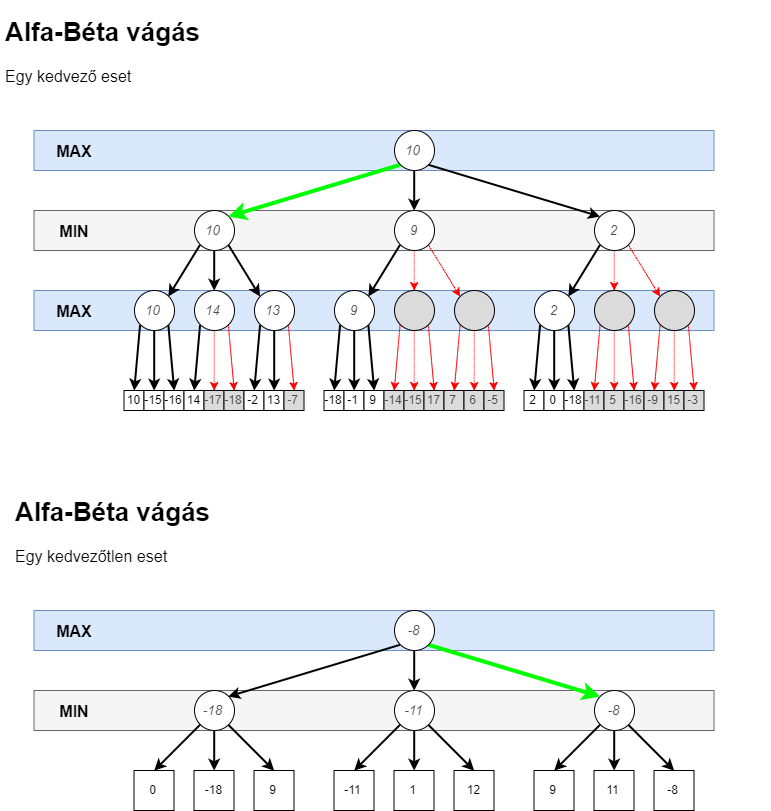
\includegraphics[width=\textwidth]{img/alphabeta_examples.png}
	\caption{Alfa-béta algoritmus számítási-igény változása a bejövő adatok sorrendjének függvényében.}
	\label{fig:alphabeta_examples}
\end{figure}

\subsection{Egy érdekes végtelen ciklus}
Vigyázni kell, mert az azonos kezdeti feltételek kombinálva azonos algoritmussal, max-mélységgel és kiértékelő függvénnyel egy végtelen játszmába vezethet. Előfordulhat, hogy a botok elkezdenek oda-vissza lépni és onnantól csak ezt a négy lépést ismételgetni. Ez a probléma a determenisztikus algoritmusoknál jöhet elő, mint például egy minimax-nál, ahol ugyanarra a bemenetre ugyanazzal a kiértékelő függvénnyel és mélységgel ugyanaz az eredmény fog kijönni a végén. Probléma lehet még például ha az egyik oldalon egy minimax, a másikon egy alfa-béta algoritmus fut, hiszen az esetek nagy többségében ezek az algoritmusok ugyanazt az eredményt adják, az alfa-béta csak a minimax egy gyorsítása.

Tehát adott 3 paraméter: algoritmus, mélység, kiértékelő függvény. Ekkor hogy elkerüljük, a végtelen-csapdát a következőket tehetjük:
\begin{itemize}
	\item \textbf{Különböző kiértékelő függvény} \\ 
	Azonos algoritmus és mélység-beállítás esetén a két botnak különböző kiértékelő függvénye legyen
	
	\item \textbf{Különböző algoritmusok} \\
	Azonos mélység-beállítás és kiértékelő függvény esetén a két botnak ne ekvivalensen determinisztikus algoritmusa legyen. (Például ne legyen minimax és alfa-béta párosítás, de például megy minimax-minimax átlagoló már működhet.)
	
	\item \textbf{Maximális mélység-beállítás legyen különböző} \\
	Azonos algoritmus és kiértékelő függvény esetén a maximális mélység-beállítás legyen különböző
	
	\item \textbf{Nem-determinisztikussá tétel} \\
	Ha mindhárom azonos, akkor pedig lehet egy kis véletlenszerűséget becsempészni akár az algoritmusba, akár a kiértékelő-függvénybe.
\end{itemize}

\section{A kiszolgáló (\texttt{Service} projekt)}
A bevezetőben már volt róla szó: mivel kérés-válasz párokra épül maga az eredeti játék is, ezért egy RESTful szolgáltatás építése tünik a legmegfelelőbbnek amely JSON-ban kommunikál. Ez azért is lesz jó, mivel így bármilyen platformon viszonylag könnyű lesz hozzá klienst írni illetve mivel iparági-sztenderd, így könnyű hozzá könyvtárakat letölteni és használni. Például a \textit{Visual Studio}-ban pár kattintással létrehozhatunk egy teljesértékű szolgáltatást egy példa végponttal, illetve felhasználó-regisztrációval, beléptetéssel.

Framework szempontjából a \textbf{.NET Core 2.1}-et használjuk, mert lehetővé teszi a cross-platform fejlesztést (lásd. .NET Standard) és így a könyvtárak más platformokon is használhatók lesznek.

Adatbázisnak \textbf{MSSQL}-t fogunk hanszálni, mert egy már fentiekben definiált \textit{Microsoft}-os fejlesztői környezetbe jól integrálódik és így könnyű vele dolgozni.

A kliens-programokhoz \textbf{WinForms} keretrendszert fogunk használni, mivel talán az egyik legegyszerűbb (habár nem a legjobb) rendszer.

A szolgáltatás weboldalát Razor engine fogja generálni, az API referencia-dokumentációjának automatikus elkészítéséhez pedig a \textbf{Swagger}-t fogjuk használni, amely segítségével még le is generálhatunk egy kliens-vázat a szolgáltatáshoz szinte bármely jelentősebb nyelvre, így könnyítve meg a jövőbeli API-felhasználó fejlesztők dolgát, akik például nem .NET-ben hanem JAVA-ban vagy akár go-ban szeretnének klienst vagy botot fejleszteni a projekthez.

\subsubsection{RESTful API}
A szerver \textbf{RESTful} szolgáltatást nyújt a kliensek felé, amely többek között azt jelenti, hogy a szerver nem tárol információt a klienssel fennálló kapcsolatról, a kliens elegendő információt kell hogy küldjön a szervernek ahhoz, hogy az válaszolni tudjon.

A kommunikáció alapjaként a HTTP protokollt fogjuk használni, amely rendelkezik a szükséges státuszjelzésekkel, így egy teljesértékű API-t tudunk nyújtani extra-munka nélkül.

További információért lásd.: \cite{restfulEn}.

\subsection{Adatbázis}
Az adatbázis felhasználók regisztrációját és beléptetését kezelő része adott, hiszen része a Microsoft .NET Core MVC alapbeállításainak, így csak a hozzá kapcsolódó és magával a sakkal foglalkozó részt kell megtervezni. Ez EF Core használata miatt elég egyszerű, hiszen C$\sharp$ osztályokból épít sémát, amelyet ha módosítás történik, karban is tud tartani. A \ref{fig:dbdiagram} ábrán láthatók a táblák és kapcsolataik.

\begin{figure}[htbp]
	\centering
	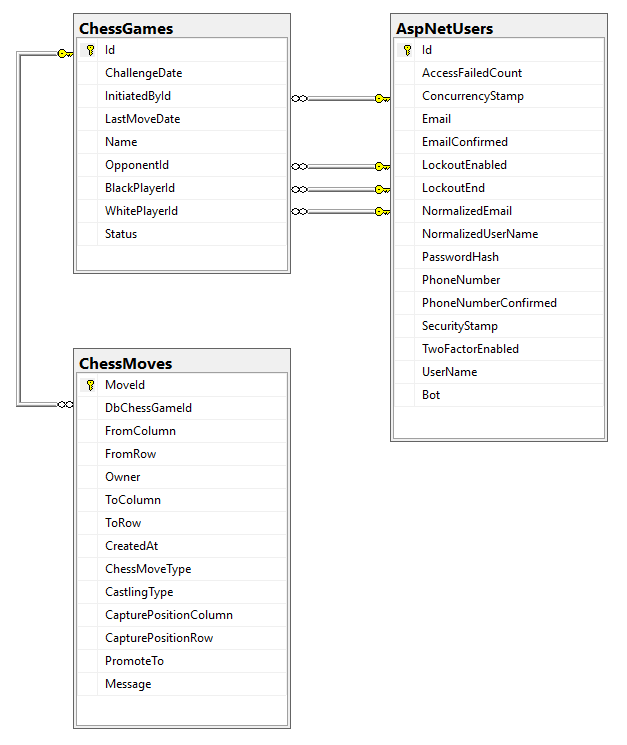
\includegraphics[width=1.0\textwidth]{img/dbdiagram.png}
	\caption{Adatbázis diagram}
	\label{fig:dbdiagram}
\end{figure}

A \texttt{ChessGame} tábla tartalmazza a partikat. Ehhez kapcsolódik a \texttt{ChessMoves} tábla, amely magukat a lépéseket tartalmazza.

Az \texttt{AspNetUsers} tábla tartalmazza a regisztrált felhasználókat, illetve ide vannak bekötve a \texttt{ChessGame} tábla olyan mezői is, mint \texttt{Opponent}, \texttt{BlackPlayer}, \texttt{WhitePlayer} és az \texttt{InitiatedBy}.

A kötések \texttt{FOREIGN KEY}-ek így biztosítják az adatbázis konzisztenciáját. (Nem lehet törölni egy entitást addig, amíg van rá hivatkozás.)

\subsection{Kommunikáció a szerver és a kliensek között}
A kommunikáció \textbf{JSON} üzenetek formájában, HTTP verb-ekkel és HTTP status kódokkal történik, ahogy a \ref{fig:clientServerCommunication} ábrán látható. Sikeres bejelentkezés során a szerver küld egy \texttt{JWT Token}-t, amelyt minden kérésnél a kliensnek mellékelnie kell a kérés fejlécében.

\subsubsection{A JWT-token (egy) problémája}
A JWT-token tartalmazza az érvényességi idejét. Alapvetően ez befolyásolja, hogy meddig használható fel, ezért amíg le nem jár, addig a szerver el is fogja fogadni. Ezért néha meg kell újítani, illetve nem visszavonható és módosítható alapból. Tehát például abban az esetben, ha egy token a következő fél órában még érvényes de a hozzá tartozó felhasználót ki akarjuk tiltani a szerverről, akkor egy "visszavonási lista" nélkül (vagy valami hasonló megoldással) ezt nem tudjuk megtenni.

Továbbá általában tartalmazza a felhasználó jogait is. Ha például egy felhasználót promótálunk, akkor a régi token még mindig a régi jogait fogja tartalmazni, ezért ha frissíteni akarjuk, akkor ki kell lépnie és vissza, hogy az újonnan kapott token már a friss információt tartalmazza a felhasználóról.

További információ a JWT token-ekről elérhető a \href{https://jwt.io/}{JWT.io} oldalon.

\subsection{Dokumentáció}
A később részletezett open-API dokumentációját a swagger nevű generátorral oldjuk meg, amely felépítését mutatja a \ref{fig:serverUiDocumentation}. ábra.

Az API dokumentációt a \textit{swagger}\cite{swaggerHomepage} generálja a kód, az annotációk és '\textit{summary}' tag-ek alapján.

A swagger generál egy az API-t leíró sémafile-t is, amelyet felhasználva a swagger oldalán generáltathatunk egy kliens a legtöbb nyelvre.

\begin{minipage}{\linewidth}
\begin{lstlisting}[caption=Health-check példakód 'summary' tag-ekkel., label=lst:healtcheck]
/// <summary>
/// The health controller. Only used to return the version information.
/// (Can only respond when the service is up and running.)
/// </summary>
[Route("api/Health")]
public class HealthController : Controller
{
	/// <summary>
	/// Health check. Returns the version number of the service.
	/// </summary>
	/// <returns>The version information of the service.</returns>
	[ProducesResponseType(typeof(string), (int)HttpStatusCode.OK)]
	[HttpGet]
	public async Task<IActionResult> Get()
	{
		var version = Microsoft.Extensions
						.PlatformAbstractions
						.PlatformServices
						.Default
						.Application
						.ApplicationVersion;

		return Ok(version);
	}
}
\end{lstlisting}
\end{minipage}
	
A fenti kódban a \texttt{Get()} függvény \textit{summary} szövege lesz az API végpont dokumentációjában, a \texttt{ProducesResponseType} attribute class-szal pedig jelezhetjük, hogy milyen HTTP státuszjelzés mellett milyen modell jön vissza a szervertől. Például: '200 OK' mellett visszajön egy várt komplex objektum, de mondjuk '500 ERROR' mellett visszajön egy komplex hibaobjektum, nem csak maga a hibakód és az esetleges hibaüzenet.

\section{Kliens-könyvtárak (\texttt{ServiceClient} projekt)}
A \texttt{ServiceClient} projektben találhatók azok az osztályok, amelyek segíthetik a fejlesztőt egy kliens írásában. Két főbb osztály van implementálva, az egyik közelebb van az API-hoz, abban segít, hogy könnyű legyen összeállítani a kéréseket. Ez a \texttt{ChessServiceClient} osztály. A másik "business object"-ként segít: ezen keresztül lehet vizsgálni az aktuális állapotát a játékos partijainak. Ezt valósítja meg a \texttt{ServiceConnection} osztály.

\section{Két példakliens}
\subsection{Sakktábla megjelenítése (\texttt{ChessBoardGamePanel})}
A \texttt{ChessBoardGamePanel}-en keresztül lehet látni a játék aktuális állapotát és ezen keresztül lehet kiválasztani a következő lépést. \texttt{OnValidMoveSelected} eseménye akkor aktiválódik, amikor egy lépés ki lett jelölve.

Az elemzés részben megemlítettük, hogy jelöléseket ragaszthatunk a bábukra, hogy gyorsítsuk egy-egy algoritmusunkat. A megjelenítéskor látható "mvd" és "ep" szavak pont ezek a jelzések. Az "mvd" jelentése "moved", azaz már elmozdult az eredeti helyéről, illetve az "ep" azt jelenti, hogy a gyalog "en passant üthető".

\subsection{A játékkliens (\texttt{HumanClient} projekt)}
A \texttt{ServiceConnection} osztályon keresztül kommunikál a szerverrel. Bizonyos időközönként frissíti a háttérben az állapotát és ha történt változás, akkor megmutatja azt.

\subsection{A botkliens (\texttt{BotClient} projekt)}
A \texttt{ServiceConnection} osztályon keresztül kommunikál a szerverrel. Bekapcsolás után folyamatosan frissíti az állapotát és ha talál olyan játékot, amelyre válaszolhat, akkor a megadott paraméterekkel kigenerálja a választ.

\section{Egyéb segédkönyvtárak (\texttt{Tools} projekt)}
E könyvtár tartalmazza azokat a komponenseket és alkalmazásokat, amelyek segítségével ki lehetett próbálni egy-egy új funkcionalitást a még készülő szoftverben.

\subsection{A \texttt{ChessboardVisualizer} osztály}
Tartalmazza a kódot a Visual Studio visualizer-hez. Sokat segít debug-olás közben, hiszen a segítségével lehet látni a sakktáblát és lehet navigálni a lépések között is.

\subsection{Algoritmus és API tesztelő alkalmazások}
Az \texttt{AlgorithmOfflineTester} és a \texttt{ChessServiceTestApp} alkalmazások a fejlesztés elején segítettek abban, hogy kipróbálhassuk: mennyire működőképes egy-egy elgondolás. További információk a függelékben \ref{proofOfConcept}.

\newpage
\chapter{Tesztelés}
A tesztelésnek különböző szintjei vannak:
\begin{itemize}
	\item \textbf{Unit tesztek} \\
	Egyszerű és gyors tesztek, általában egy kisebb egységet: metódust, függvényt tesztel. Ebben a szoftverben főleg a központi elemeket, a reprezentációt és a mechanizmust teszteli hiszen központi részei a dolgozatnak. Ha ezek nem működnek megfelelően, akkor az egész programcsomag nem működik megfelelően.
	
	\item \textbf{Integrációs tesztek} \\
	A rendszer különböző komponenseinek együttműködését teszteli. Technológiai szemszögből néz a problémára: nem feladata a helyesség megállapítása, a komponensek közötti együttműködést vizsgálja. Könnyen elkészíthető, hiszen a .NET Core rendelkezésünkre bocsájt egy \texttt{TestServer} nevű osztályt, amely memóriában futva szimulálja az alrendszereket.
	
	\item \textbf{API tesztek} \\
	Ettől a szinttől felfelé már a helyesség is fontos. A kiajánlott API tesztelésekor a publikus API felületet hívjuk meg előre definiált adatokkal és figyeljük a működést.
	
	\item \textbf{GUI tesztek} \\
	Ezek lehetnek automatikus vagy manuális tesztek. Többnyire utóbbit szokták választani, mert egy gyorsan változó környezetben nagyon nehéz a teszteket módosítani és validálni.
	
	\item \textbf{Teljesítmény-teszt} \\
	Automatikus teszt, ahol a rendszert hatalmas bejövő adatnak teszik ki és figyelik a viselkedését, különösképpen arra, hogy leáll-e, elfogy-e a CPU vagy a memória, esetleg megjelennek-e deadlock-ok, illetve okoz-e anomáliákat a többi rendszerben.
	
	\item \textbf{Rendszerteszt} \\
	Manuális teszt, ahol felállítanak egy tesztkörnyezetet és megpróbálják szimulálni a mindennapos használatot.
	
\end{itemize}

Felülről lefelé haladva nő ezen tesztek ára és komplexitása. Jelen dolgozatban időhiány miatt csak unit és manuális tesztek vannak, de az automatikusan válaszoló botokkal a rendszert így is meg lehetett tesztelni (integrációs-, teljesítmény- és API teszt), amely fel is fedett jó néhány hibát.

\section{Reprezentáció}
A tesztelés unit-teszteken keresztül történik, amelyben előre megadott szituációkat mutatva a kódnak megvizsgáljuk, hogy a lehetséges lépéseket kapjuk-e meg vagy sem, illetve manuálisan végignézve állásokat megállapítjuk, hogy jók-e az állások. Egy sakk-matt tesztelő példát láthatunk a \ref{lst:checkmate_test} kódrészletben.

\begin{lstlisting}[caption=Sakk-matt detektálás teszt, label=lst:checkmate_test, float]
[Fact]
public void GameStateCheck_CheckMateTest_BlackWins()
{
	var expected = GameState.BlackWon;
	
	// Fool's mate
	var game = new ChessRepresentationInitializer().Create();
	var mechanism = new ChessMechanism();
	var moves = new List<BaseMove>(4)
	{
		new ChessMove(ChessPlayer.White, Positions.G2, Positions.G4),
		new ChessMove(ChessPlayer.Black, Positions.E7, Positions.E5),
		new ChessMove(ChessPlayer.White, Positions.F2, Positions.F3),
		new ChessMove(ChessPlayer.Black, Positions.D8, Positions.H4)
	};
	
	foreach (var move in moves)
	{
		game = mechanism.ApplyMove(game, move);
	}
	
	var actual = mechanism.GetGameState(game);
	
	Assert.Equal(expected, actual);
}
\end{lstlisting}
\subsection{Kiterjesztések}
A sakktáblán való navigáláshoz készült sok segédfüggvény is, hogy könnyebben lehessen navigálni illetve egyik formátumból a másikba konvertálni, illetve az olyan segédfüggvényekhez is, mint az "északra kettőt", "lólépés" satöbbi.

\subsection{Külön vizsgálandó esetek}
Főleg a különleges lépéseket kellett jól letesztelni. Például:
\begin{itemize}
	\item \textbf{Sáncolás} Nagyon szigorú szabályok vannak arra, mikor lehet sáncolni. Ezeket az eseteket végig kellett venni.
	
	\item \textbf{Sakk-matt} A tesztek között van két nevezetes sakk-matt szituáció: a suszter-matt és a bolond-matt. Egyiket a világos, a másikat a sötét játékos kaphatja.
	
	\item \textbf{Speciális lépések} Például Feladás, döntetlen felajánlása, stb.
	
	\item \textbf{En passant} En passant lépés tesztelése.
	
	\item \textbf{Promóció}Amikor a gyalog átér, akkor átváltozik egy tiszté.
\end{itemize}

\subsection{Visual Studio Visualizer}
A unit-tesztek írása közben sok hiba jött elő és sokat közülük nehéz volt kijavítani, mert nagyon nehéz elképzelni, hogy mi is történik éppen. Ezért ki lett fejlesztve egy \textbf{Visualizer} a \texttt{ChessRepresentation} osztályhoz, amely beépül a Visual Studio-ba és ott ha debug közben rávisszük a kurzort az objektumra, akkor megnézhetjük vizuálisan is a sakktáblát, illetve oda-vissza lépkedhetünk a történetében is. Ez a projekt része, habár fordítás után be kell másolni a \texttt{C:\textbackslash Users\textbackslash FELHASZNÁLÓNÉV\textbackslash Documents\textbackslash Visual Studio 2017\textbackslash Visualizers\textbackslash} könyvtárba és egy VS újraindítás után már használható. Ez látszik a \ref{fig:visualizer} ábrán.

\begin{figure}[htbp]
	\centering
	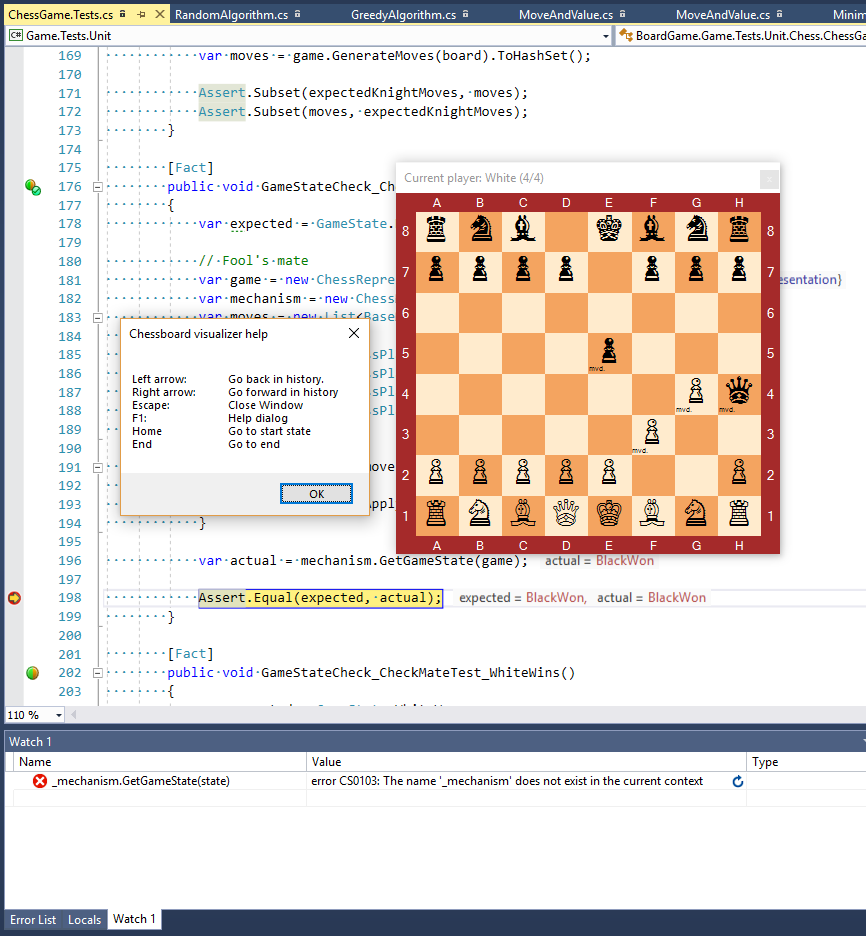
\includegraphics[width=0.7\textwidth]{img/visualizer.png}
	\caption{Visualizer működés közben, a súgó ablakával nyitva.}
	\label{fig:visualizer}
\end{figure}

\subsection{Manuális tesztelés játék közben}
Sok szituáció volt kipróbálva manuális játék közben is, ahol két klienst futtatva mindkettőbe bejelentkezve különböző szituációkat előidézbe teszteltem a játékot. Ezt end-to-end tesztnek is vehetjük, hiszen a játék-infrastruktúra minden elem le lett ezáltal tesztelve, illetve speciális helyzeteket előidézve a játéklogika is:
\begin{itemize}
	\item Sáncolás tesztelése,
	\item En passant tesztelése,
	\item Promóció minden bábutípusra, külön figyelve arra, hogy az átváltozás okoz-e sakkot,
	\item Patt helyzet előállítása, a kód felismeri-e
\end{itemize}

\section{Algoritmusok}
A tesztelés unit-teszteken keresztül történik, amelyben előre megadott adatokra azt kapjuk-e, amit elvárunk. Példa unit teszt látható a \ref{lst:greedy_test}. kódrészletben.

\begin{lstlisting}[caption=Mohó-algoritmus teszt, label=lst:greedy_test, float]
[Fact]
public void Test1()
{
	var evaluator = new TestCase1.Evaluator();
	var generator = new TestCase1.Generator();
	var applier = new TestCase1.Applier();
	var algorithm = new GreedyAlgorithm<TestCase1.State, TestCase1.Move>(evaluator, generator, applier);
	
	var initState = new TestCase1.State(0, 0);
	
	var move1 = algorithm.Calculate(initState);
	var state2 = applier.Apply(initState, move1);
	var move2 = algorithm.Calculate(state2);
	
	Assert.Equal('a', move1.Label);
	Assert.Equal('d', move2.Label);
}
\end{lstlisting}

Ezekkel a tesztekkel az a probléma, hogy nagyon nehéz őket összeállítani: fel kell építeni egy reprezentációt, majd abban megírni egy kiértékelő osztályt, egy generátor osztályt. Rengeteg a hibalehetőség. Ezért inkább a manuális tesztek felé fordultam:
Először a botokat játszattam egymással és figyeltem, hogy lefagynak-e, rosszat lépnek-e, mekkora a memória és CPU igényük. Végül elkezdtem ellenük játszani.

\subsection{Szolgáltatás}
Az infrastruktúra tesztelését manuális játékkal illetve a botok közötti játékkal lehetett kvázi-automatikusan tesztelni. Erre volt jó például a véletlen-algoritmus és a mohó-algoritmus, hiszen nagyon gyorsak, így elég sok lépést meg tudnak tenni viszonylag rövid idő alatt.

\subsection{API}
POSTMAN használatával történt az API hívások tesztelése. Mivel HTTP-n keresztül, JSON-ben megy a kommunikáció, ezért könnyű volt a különböző eseteket összállítani és letesztelni minden esetet. (Bad request, autentikációs probléma, stb.) Később a botok egymás elleni játéka illetve emberi játékosok egymás és botok elleni játéka által is tesztelve volt az API és fel is derített néhány hibát.

\subsection{Szerver UI}
A szerver oldalon minimális UI van, ezért nincs szükség túl sok manuális tesztelésre. Amit meg kellett nézni:
\begin{itemize}
	\item Mi történik, ha nem megfelelő a megadott jelszó?
	\item Mi történik, ha regisztrációkor az egyik megadott adat nem megfelelő?
	\item Elérhetők-e a letölthető file-ok és a dokumentáció?
\end{itemize}

\section{Játékkliens}
Elejétől a végéig manuális teszteléssel.
\begin{itemize}
	\item Mi történik rossz jelszó megadásakor?
	\item Mi történik, ha nem megy a szerver? Jól kezeli a kliens?
	\item Mi történik, ha akkor próbálok lépni, amikor nem az én köröm van? Mi van, ha nem megengedett lépést akarok beküldeni?
	\item Mi történik normál esetben?
	\item Mi történik, ha a szerver leterhelt és lelassul?
\end{itemize}

\section{Botkliens}
Az infrastruktúra tesztelésekor önmagát is tesztelte. Ugyanazon aspektusokból kellett tesztelni, mint a játékklienst.
\begin{itemize}
	\item Mi történik rossz jelszó megadásakor?
	\item Mi történik, ha nem megy a szerver? Jól kezeli a kliens?
	\item Mi történik, ha akkor próbálok lépni, amikor nem az én köröm van? Mi van, ha nem megengedett lépést akarok beküldeni?
	\item Mi történik normál esetben?
	\item Mi történik, ha a szerver leterhelt és lelassul?
\end{itemize}

\section{Megfigyelések}
\subsection{Algoritmusok sebességkülönbsége}
Az alfa-béta algoritmus egy jelentős gyorsítása a minimax algoritmusnak. Megfigyelések alapján körülbelül fele annyi idő kellett neki, hogy kiszámolja ugyanazt a mélységű eredményt. 

\subsection{Hamis biztonságérzet}
Nem megfelelő unit-teszt lefedettség mellett ha a tesztelendő algoritmusaink bonyolultak, akkor az adhat egy hamis-biztonságérzetet, hogy "ad valamilyen eredményt". Ez nagyon veszélyes, hiszen ha nincsenek letesztelve a szélsőséges esetek, akkor előfordulhat, hogy az algoritmus nemhogy rossz, hanem semmilyen eredményt sem fog adni.

\subsection{Erőforráshiány}
Egy idő után lehetetlenné vált a tesztelés a lokális gépen, mert a sok bot kliens, a service, az adatbázis szerver illetve a Visual Studio együttesen már annyira leterhelte a gépet, hogy lehetetlenné vált minden a munka a gépen. Ezért lett a project publikálva egy külső szerverre.




% ============================================================================================================
% === FÜGGELÉK ===============================================================================================
% ============================================================================================================
\newpage
\part{Függelék}
\chapter{Néhány érdekesség a sakkról}
\section{Játékok osztályozása}
A \textbf{„kétszemélyes, teljes információjú, diszkrét, véges és determinisztikus, zéró-összegű, játékok”} definíciója egy kis magyarázatot érdemel. A játékokat a kövektező szempontok alapján lehet osztályozni:

\begin{itemize}
	\item \textbf{Játékosok száma} \\
	Ez lehet egy, kettő, vagy n.
	
	\item \textbf{Elérhető információ mennyisége} \\
	A játékosok számára mennyi információ érhető el? Minden információ birtokában vannak-e (pédlául sakk), vagy nem (például egy kártyajáték, ahol nem látják egymás lapjait.)
	
	\item \textbf{Körökre-osztott-e vagy sem?} \\
	Lépések diszkrét sorozatából áll-e a játék vagy folyamatos.
	
	\item \textbf{Lehetséges lépések száma} \\
	Diszkrét esetben a különböző állapotokban lehetséges lépések száma véges vagy végtelen? A játék véges sok lépésben végetér?
	
	\item \textbf{Véletlen-faktor} \\
	A véletlennek van-e szerepe a játékban? Ha nincs, akkor a játékot \textit{determinisztikusnak} hívjuk.
	
	\item \textbf{Játékosok nyereségeinek összege} \\
	Ha a játékosok nyereségeinek összege 0 (amennyit nyer az egyik, annyit veszít a másik), akkor \textit{zérusösszegű} a játék.
\end{itemize}

Ez alapján a sakk egy:
\begin{itemize}
	\item \textbf{Kétszemélyes}
	
	\item \textbf{Tejes információjú} \\
	Ránézve a sakktáblára és a játéklépések jegyzékére minden játékos tudja a pontos állást.
	
	\item \textbf{Diszkrét} \\
	Mert diszkrét lépések sorozata egy játék.
	
	\item \textbf{Véges} \\
	Mivel véges sok lépésben végetér a játék és az állapotokból lehetséges lépések száma is véges.
	
	\item \textbf{Determinisztikus} \\
	Mivel a szerencsének nincs szerepe a játékban.
	
	\item \textbf{Zéró-összegű} \\
	A szerzett pontok száma mindig egy: győztes játékos 1 pontot kap, a vesztes 0-t, döntetlen esetén 0.5-0.5 pontot kapnak a felek.
\end{itemize}
játék.

\section{A sakk története}
A játék neve a perzsa „shāh” szóból ered, amely uralkodót jelent.\footnote{A "sakk-matt" kifejezés pedig a perzsa „Shāh Māt" kifejezésből származik, amelynek jelentése: "a királyt lerohanták” vagy "védtelen”, "legyőzött”.\cite{ChessMateHu}\cite{ChessMateEn}} Története a legendák világába nyúlik vissza. Egy ismert mese szerint egy brahmin találta ki a sakkot. Jutalmul a rádzsától első hallásra jelentéktelennek tűnő fizetséget kért, mindössze annyi búzaszemet, amennyi a sakktábla kockáira a következő szabály szerint képletesen rátehető: az első kockára egy, a másodikra kettő, a harmadikra négy, vagyis az előzőnek mindig duplája. Hamar kiderült, hogy ennyi búza nem terem a Földön, sőt az emberiség egész történelme alatt nem termelt ennyit.

Az első ismert változata valószínűleg Indiában alakult ki. A maihoz képest egyszerűbb volt, de ugyanakkora táblán és ugyanazokkal a bábukkal játszották, a lépések viszont különböztek. 

Indiából először Perzsiába jutott el. Amikor az arabok elfoglalták Perzsiát, a muszlim világ átvette és ennek következményeként el is terjesztette a játékot Dél-Európában. A sakk mai formáját körülbelül a XV.-ik században érte el.

Keleti terjedése már kissé bizonytalan: először Kínába majd Japánba jutott el és közben sokkal nagyobb változásokon ment keresztül.
\textit{Egy kevésbé elfogadott elmélet szerint eredetileg Kínából származik és terjedt el.}\cite{HistoryOfChessHu}\cite{HistoryOfChessEn}

\section{Egy "gondolkodó gép": a Török}
\begin{wrapfigure}{l}{5cm}
	\caption{Kempelen Farkas - A Török}
	\label{fig:the_turk}
	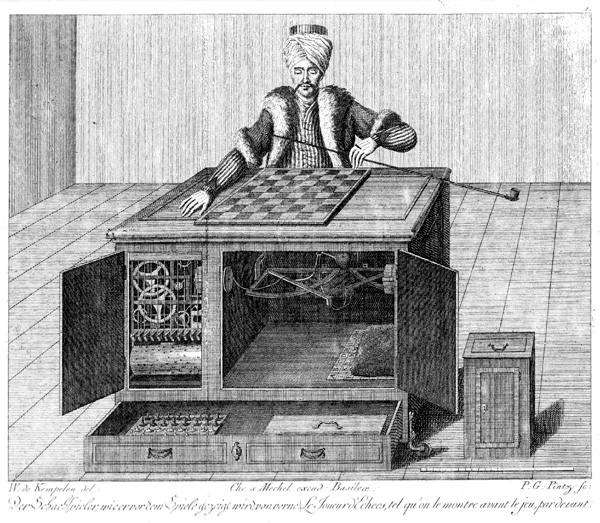
\includegraphics[width=5.0cm]{img/the_turk}
\end{wrapfigure}
A Török Kempelen Farkas által 1769-ben alkotott legendás sakkozógép volt, melyet azért épített, hogy elkápráztassa vele Mária Teréziát. A gép sakkpartikat játszott és nyert. Végül végigtúrázta Európát és Észak-Amerikát míg 1854-ben Philadelphiában egy tűzben meg nem semmisült. 

A gép titka nem egy zseniális korát meghaladó "mechanikus mesterséges intelligencia" volt, hanem egy benne elrejtőző emberi kezelő. Ez a gyanú többször is felvetődött, de Kempelen a játszmák előtt felnyitva a gépet mutatta be, hogy nincs senki a gépben. Valójában az eléggé apró termetű kezelő el tudott bújni, amíg elöl illetve hátul is kinyitották a szerkezetet, hogy belenézhessenek. A gépet végül 1857-ben leplezte le nyíltan a The Chess Monthly című amerikai sakklap.\cite{MechanicalTurkHu}\cite{MechanicalTurkEn}\cite{CsodakKonyveHu}

\section{Kaissza}
Az 1950-es évektől kezdődően egyre több, egyre erősebb sakkprogramot írtak. 1947-ben készült el a világ első sakk-komputer programja, amelyet Alan Turing írt. 1974-ben volt az első sakkprogram-világbajnokság, ahol a győztes a szovjet Kaissza(\foreignlanguage{russian}{Kaissa}) nevű program volt, amely 1974 és 1977 között uralta a nemzetközi számítógépes sakkot.\cite{chessProgramsHu}

1990-ben elkészíteték PC-s verzióját, amely a londoni számítógépes olimpián negyedik helyezett lett.\cite{KaissaEn}
\newline \\
\section{Deep Blue}
\begin{wrapfigure}{r}{5cm}
	\caption{Deep Blue}
	\label{fig:deepblue}
	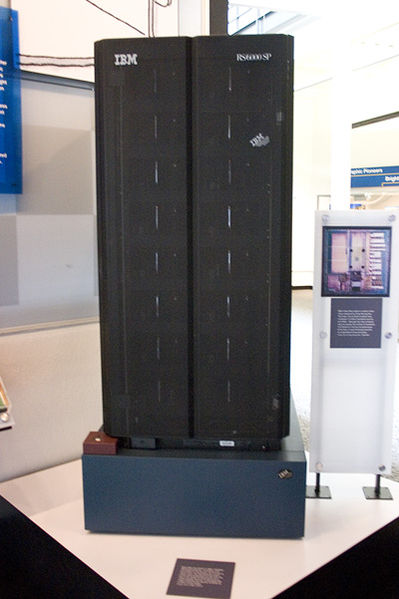
\includegraphics[width=5.0cm]{img/deepblue.jpg}
\end{wrapfigure}
A Deep Blue az IBM által körülbelül 20 millió dolláros költséggel kifejlesztett számítógépe, amely sakkjátékban 1997-ben egy szabályszerű hatjátszmás páros mérkőzésen New Yorkban legyőzte Garri Kaszparovot, az emberi sakkozás akkori világbajnokát.

Első meccs-győzelmét 1996 február 10.-én érte el a világbajnok ellen, de Kasparov három partit nyert és kettőt hozott ki döntetlenre, így 4-2-re győzött a számítógép ellen.

Ezután Deep Blue-t továbbfejlesztették és ekkor már 3,5–2,5-re verte Kasparov-ot 1997 májusában, és ezzel az első számítógépes rendszer lett, amely meg tudta verni az aktuális sakk-világbajnokot a sakkbajnokságokra jellemző időmegszorítás mellett. Kasparov csalást gyanított, és követelt egy visszavágót, ám ebbe az IBM nem ment bele. \cite{DeepBlueHu}\cite{DeepBlueEn}

\chapter{Egyéb segédprogramok}\label{proofOfConcept}
\section{Az algoritmus-teszter}
Az algoritmusok egymás elleni tesztjében lehet segítség egy egyszerű alkalmazás, amelyben az algoritmusokat különböző beállításokkal egymásnak lehet engedni a szerver kihagyásával. Az alkalmazás nagyon egyszerű és nem "prodution ready". A solution-ben \texttt{OfflineAlgorithmTester} néven található, \ref{fig:offlineAlgorithmTester}. ábrán látható a főképernyője.

\begin{figure}[htbp]
	\centering
	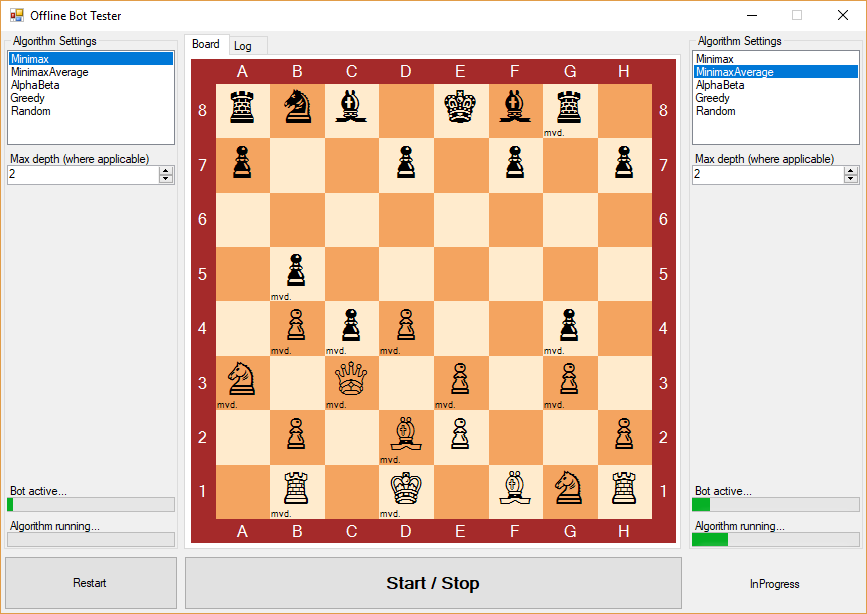
\includegraphics[width=1.0\textwidth]{img/offlineAlgorithmTester.png}
	\caption{Algoritmusok tesztelése egymás ellen}
	\label{fig:offlineAlgorithmTester}
\end{figure}

\section{Szolgáltatást tesztelő alkalmazás}
Még a fejlesztés elején készült, hogy ki lehessen próbálni az API-hívásokat, illetve lehessen elemezni a sakkjátszmákat. Ez sem "production-ready", a kódminősége is mutatja: inkább csak amolyan "proof-of-concept". A solution-ben \texttt{ChessServiceTestApp} néven található, \ref{fig:chessClientTesterApp}. ábrán látható a főképernyője.

\begin{figure}[htbp]
	\centering
	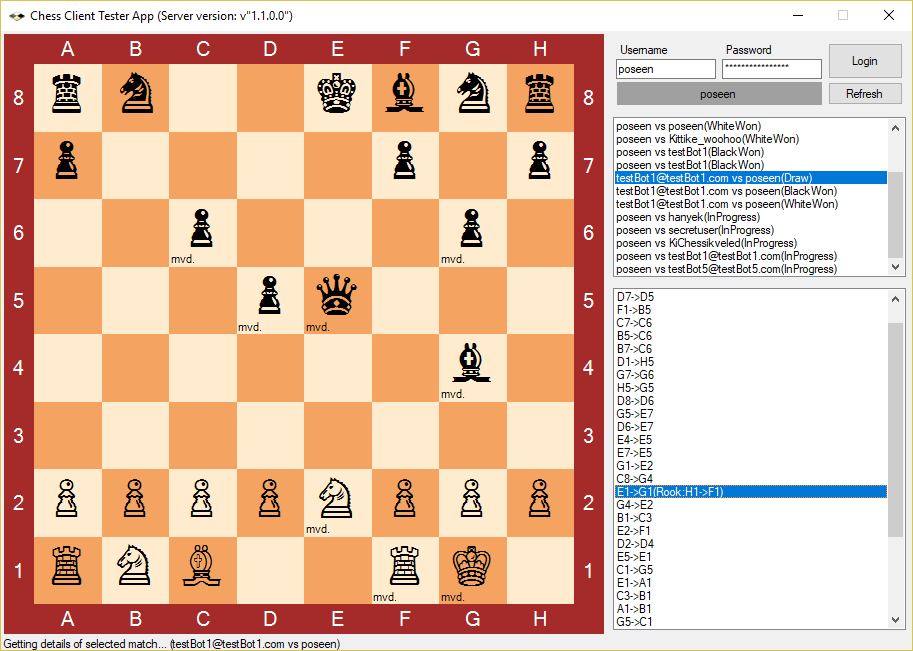
\includegraphics[width=1.0\textwidth]{img/chessClientTesterApp.png}
	\caption{A szolgáltatást tesztelő alkalmazás}
	\label{fig:chessClientTesterApp}
\end{figure}

\section{"Proof of Concept"}
Ezen programok jellemzője, hogy csak belső használatra készültek a programcsomag fejlesztésének elején, hogy minél előbb látszódjon, ha egy koncepció működik, vagy nem működik. Ezt hívjuk "\textbf{proof of concept}"-nek, avagy röviden "\textbf{POC}"-nek. Ezekkel szemben nem elvárás a jó kódminőség vagy a felhasználóbarátság, bár nem is tiltott természetesen. Célja az, hogy be lehessen mutatni: amit kitaláltunk az egy működőképes koncepció. Általában új termékek vagy ötletek bevezetésénél szoktak ilyet írni nagyon rövid idő alatt, így minimalizálva a veszteséget abban az esetben, ha a POC azt mutatja, hogy mégsem működhet a koncepció vagy a megrendelőnek nem tetszik.

\subsection*{Murphy törvénye}
Ami elromolhat, az el is romlik. Nincs száz százalékos bizonyosság sosem. Hiába a rengeteg manuális vagy automatikus teszt, a program valamely része mindig akkor és ott romlik el, amikor és ahol a legkevésbé számítunk rá, főleg ha egy olyan bonyolult rendszerről van szó, mint egy mesterséges intelligencia algoritmusáról, amely működése kívülálló szemszögéből nem egyértelmű. Megfigyelt jelenség, hogy a betonbiztosan működő szoftver is általában a megrendelő számára tartott bemutató előtt összeomlik. Ezért mindig legyen B-tervünk. És egy C.

\section{Fordított CAPTCHA}
Felmerült egy érdekes probléma a kliensprogramok tervezése során. Minden ilyen rendszer fejlesztésekor gondolni kell a rosszindulatú felhasználásra, jelen esetben például arra, mi van akkor és hogy szűrhető ki, ha valaki csalni akar. Többféle módja van a csalásnak, azonban van két eset, amely külön érdekes:
\subsection*{Rossz sakkozó, de erős programozó}
Az egyik az, ha valaki nem jó sakkozó, de tud jó programot írni. Ekkor felmerülhet az ötlet, hogy amikor egy másik játékos ellen játszik, akkor erre az esetre ír egy programot, amelyikbe betáplálva a lépéseket az egy olyan lépést mutat, amit esetleg a játékos magától nem lépett volna, ezáltal hozzásegítve egy jobb helyezés eléréséhez.

Ez a probléma nem ismeretlen a levelezési-sakk világban, és igazából elfogadják. Megfigyelések szerint jelentősen nem befolyásolja a játékok kimenetelét, inkább csak a különbséget csökkenti a kezdő és haladó játékosok között. \cite{corrChessHelpHu} Kérdés, hogy ez mennyire teszi tönkre a játékélményt, de ez inkább morális kérdés, mint a dolgozathoz szorosan kötődő technológiai.

\subsection*{Jó sakkozó, de gyenge programozó}A másik - és számunkra érdekesebb eset, - hogy mi van akkor, ha valaki jó sakkozó, de nem tud jó programot írni. Ekkor lehetséges az, hogy regisztrál egy bot felhasználói fiókot és azon keresztül játszik. Mivel mindenki a neten otthonról játszik, ezért itt sem ellenőrizhető, hogy a lépést egy bot vagy egy ember találta-e ki. A válasz erre talán egy \textbf{fordított CAPTCHA} lenne, amellyel lehetne ellenőrizni, hogy a lépéseket tényleg egy gépi intelligencia hozta-e meg, vagy egy ember. Hívhatjuk \textbf{fordított Turing-tesztnek} is. Vajon lehet-e olyan programot írni, amely eldönti egy interakcióról, hogy az géptől jön-e. Lehet-e a kaotikus emberi viselkedést majdnem pontosan detektálni és a szuperkomplex gépi interakciótól megkülönböztetni? Felismerhető-e, ha egy ember megpróbálja imitálni egy bot viselkedését?




% ============================================================================================================
% === IRODALOM - ÁBRAJEGYZÉK
% ============================================================================================================
\backmatter
\bibliographystyle{unsrt}
%\part{\bibname}
%\renewcommand{\bibname}{Irodalomjegyzék}
\bibliography{szakdolgozat}
%\addcontentsline{toc}{part}{\bibname}
%\printbibliography[heading=none]
%\newpage

\end{document}